\documentclass[class=book, crop=false, oneside, 12pt]{standalone}
\usepackage{standalone}
\usepackage{../../style}
\usepackage{../../style_automata}
\graphicspath{{./assets/images/}}

\begin{document}

\chapter{Analisi Lessicale e Linguaggi Regolari}

\section{Introduzione}

Ora che abbiamo acquisito dei mezzi più potenti per affrontare questo corso, ribadiamo il concetto di analisi lessicale: dato il programma in ingresso, l'analisi lessicale restituisce una lista di stringhe che corrisponde alle parti del linguaggio identificate; questa lista di stringhe è nota come \emph{flusso dei token}.

Lo studio del capitolo precedente di consente di sapere come vengono generati linguaggi come il seguente:

\begin{equation}
    \label{a^nb^n}
    \{ a^n b^n \mid n > 0 \}    
\end{equation}

Come detto in passato, un liguaggio con questa forma può essere utilizzato, ad esempio, nel caso in cui vogliamo avere un egual numero di parentesi aperte e chiuse.
Il problema che vogliamo arrivare a risolvere è, più in generale, riconoscere se una stringa faccia parte o meno del linguaggio generato da una certa grammatica.

Ad esempio, per affrontare il problema del linguaggio \ref{a^nb^n} viene naturale l'utilizzo di una struttura di tipo stack:

\begin{enumerate}
    \item leggiamo i simboli uno alla volta e li inseriamo nel nostro stack;
    \item per ogni \(a\) che leggiamo, inseriamola nella pila;
    \item se troviamo una \(b\), allora facciamo un pop dalla pila;
    \item se ad un certo punto stiamo tentando di togliere un elemento da una pila vuota o se, finita l’analisi, rimangono ancora elementi nella pila, allora c’è qualche errore;
    \item nel caso in cui al termine dell’analisi è andato tutto liscio e abbiamo svuotato la pila, allora la parola analizzata appartiene al linguaggio \ref{a^nb^n}.
\end{enumerate} 

La precedente strategia sicuramente è ottima quando il linguaggio ha una forma simile all'esempio che abbiamo considerato. Ma consideriamo invece la grammatica che genera tutte le parole dell’alfabeto:

\begin{equation}
    \label{alfabeto}
    S \to a \mid b \mid … \mid z \mid aS \mid bS \mid … \mid zS
\end{equation}

Per riconoscere parole generate da una tale grammatica il metodo di analisi naturale è una macchina a stati come quella in figura \ref{macchina_a_stati_finiti}.

\begin{figure}[htb]
	\centering
	\subimport{assets/figures/}{msf.tex}
    \caption{Macchina a stati finiti}
	\label{macchina_a_stati_finiti}
\end{figure}

\noindent Il funzionamento di questi strumenti di analisi ci sarà ben più chiaro in seguito.

La grammatica che produce tutte le lettere dell’alfabeto (il linguaggio \ref{alfabeto}) è una grammatica libera, ma ha anche una caratteristica in più: è regolare. Andiamo a capire meglio di cosa si tratta.


\section{Grammatiche regolari}

Le grammatiche regolari sono un sottoinsieme delle grammatiche libere che rispetta le seguenti restrizioni rispetto alle loro produzioni:

\begin{itemize}
    \item o il body è un solo terminale (\(A \to a\));
    \item o il body è composto da un terminale e un non-terminale, nella seguente forma: \(A \to aB\);  
    \item altrimenti, il body è la parola vuota (\(A \to \varepsilon\)).
\end{itemize}

Queste grammatiche possono generare espressioni regolari, che introdurremo a breve; inoltre, i linguaggi generati da queste grammatiche sono riconosciuti dagli automi a stati finiti, sia deterministici che non deterministici.

Queste due osservazioni sono la base fondante dell'utilizzo delle grammatiche regolari per l’analisi lessicale.

\subsection{Espressioni regolari}
Prima di tutto partiamo con il definire una grammatica regolare.\\
Sia fissato un alfabeto \(\mathcal{A}\) da cui estrarre tutte le basi e sia fissato un certo numero di operatori.

Le espressioni regolari sono esprimibili tramite il meccanismo dell'induzione in questo modo.
\begin{description}
    \item[Base] Sono un'espressione regolare tutti i simboli dell’alfabeto che abbiamo scelto; in aggiunta a questi, anche \(\varepsilon\) lo è, indipendentemente dall'alfabeto scelto.
    \item[Step] Se \(r_1\) e \(r_2\) sono espressioni regolari allora:
    \begin{itemize}
        \item \(r_1 \mid r_2\) è un’espressione regolare, detta \emph{Alternation};
        \item \(r_1 \cdot r_2\) è un’espressione regolare, scritta anche come \(r_1 r_2\) e detta \emph{Concatenation};
        \item \(r_1\)\(^\ast\) è un’espressione regolare che significa ripetizione di \(r\) per un certo numero \(k\) di volte, detta \emph{Kleene star};
        \item \((r_1)\) è un’espressione regolare; è usata per definire l’ordine di svolgimento delle operazioni ed è detta \emph{Parentheses}.
    \end{itemize} 
\end{description}

\subsection{I linguaggi delle espressioni regolari}
Se un linguaggio può essere ricavato da un'espressione regolare si dice che l'espressione \emph{denota} quel linguaggio; si presti attenzione a non utilizzare il termine \emph{generare}, poiché quest'ultimo è riservato per le grammatiche generative.

Detto ciò, come capiamo qual è il linguaggio denotato da un’espressione regolare?
Consideriamo un’espressione regolare \(r\) su \(\mathcal{A}\) , il linguaggio denotato da quell'espressione \(\mathcal{L}(r)\) è anch'esso definibile tramite induzione:
\begin{description}
    \item[Base] \begin{itemize}
                    \item \(\mathcal{L}(a) = \{a\} \; \forall a \in \mathcal{A}\)
                    \item \(\mathcal{L}(\varepsilon) = \{\varepsilon\}\)
                \end{itemize}
    \item[Step] \begin{itemize}
                    \item se \(r = r_1 \mid r_2 \) \\
                    allora \(\mathcal{L}(r)= \mathcal{L}(r_1) \cup \mathcal{L}(r_2)\)
                    \item se \(r=r_1 r_2\) \\
                    allora \(\mathcal{L}(r) = \{w_1 w_2 \mid w_1 \in \mathcal{L}(r_1) \land w_2 \in \mathcal{L}(r_2)\}\)
                    \item se \(r = r_1\)\(^\ast\) \\
                    allora \( \mathcal{L}(r) = \{ \varepsilon \} \cup \{ w_1 w_2 ... w_k \mid k \ge 1 \land \forall i : 1 \le i \le k.w_i \in \mathcal{L}(r_1)\} \)
                    \item se \(r=(r_1)\) \\allora \( \mathcal{L}(r) = \mathcal{L}(r_1)\)
                \end{itemize}
\end{description}

\noindent Osserviamo ora quali sono le regole di precedenza per gli operatori appena descritti.

\begin{itemize}
    \item La Kleene star ha la precedenza maggiore;
    \item La concatenazione è seconda in ordine di precedenza;
    \item L'alternanza ha la minor precedenza.
\end{itemize}

\noindent Tutte queste operazioni hanno associatività a sinistra.
Ecco un esempio esplicativo:

\begin{equation*}
    a \mid b c^\ast
\end{equation*}

\noindent Una volta applicate le regole di precedenzam, l'espressione si legge in questo modo:

\begin{equation*}
    (a \mid ( b  ( c^\ast ) ) )
\end{equation*}    

\subsubsection{Esercizi sulle operazioni con espressioni regolari}
Ecco presentati in veloce sequenza una serie di semplici esercizi sulle operazioni con grammatiche regolari. 

\begin{itemize}
    \item \(\mathcal{L}(a \mid b) = \{a, b\}\)
    \item \(\mathcal{L}((a \mid b) (a \mid b)) = \{aa, ab, ba, bb\}\)
    \item \(\mathcal{L}(a^*) = \{a^n \mid n \ge 0\}\)
    \item \(\mathcal{L}(a \mid a^\ast b) = \{a\} \cup \{a^n b \mid n \ge 0\}\)
    \item \( (a \mid b \mid \ldots \mid z)(a \mid b \mid \ldots \mid z)^\ast \) denota l’insieme di tutte le parole dell’alfabeto
    \item \( (0 \mid 1)^\ast \) denota l’insieme di tutti i numeri binari pari
    \item \( b^\ast (abb^\ast )^\ast ( a \mid \varepsilon ) \) denota l’insieme delle parole su \(\{a,b\} \), senza alcuna occorenza consecutiva di \(a\)
    \item \( (a \mid b)^\ast aa(a \mid b)^\ast \) denota l’insieme delle parole su \( \{a,b\} \) in cui ci sono sicuramente delle occorrenze consecutive di \(a\) (date da \(aa\) in posizione centrale)
\end{itemize}

\section{Automa a stati finiti}
Gli automi a stati finiti sono usati per decidere se le parole appartengono ad un linguaggio denotato da una certa espressione regolare.
Vedremo due tipi diversi di automa a stati finiti: deterministico e non deterministico; di questi tipi poi studieremo i casi di utilizzo ottimali.

Nel caso di automa a stati finiti non deterministico i calcoli sono spesso più pesanti, perché un automa non deterministico deve vagliare più perocrsi di derivazione rispetto ai loro colleghi deterministici, i quali hanno il vantaggio di dover vagliare solo i percorsi deterministici, che sono un sottoinsieme del totale.

\section{Automa a stati finiti non deterministico}
Un automa a stati finiti non deterministico (NFA) è rappresentabile con una tupla
\begin{equation*}
    \mathcal{N} := (S, \mathcal{A}, \textrm{move}_n, s_0, F)
    \label{nfa_tupla}
\end{equation*}
in cui:
\begin{itemize}
    \item \(S\) è un insieme di stati;
    \item \(\mathcal{A}\) è un alfabeto con \(\varepsilon \notin \mathcal{A}\);
    \item \(S_0 \in S\) è lo stato iniziale;
    \item \(F \subseteq S\) è l’insieme degli stati finali o accettabili;
    \item \(\textrm{move}_n : S \times (\mathcal{A} \cup \{\varepsilon\}) \to 2^S\) è la funzione di transizione: da un certo stato e con un certo simbolo (che può essere anche \(\varepsilon\)), mi muovo in un certo stato compreso nei sottoinsiemi di \(S\).
\end{itemize}

\subsection{Rappresentazione grafica}
La tupla \((S, \mathcal{A}, \textrm{move}_n, s_0, F)\) può essere rappresentata con un grafo diretto seguendo queste convenzioni:
\begin{itemize}
    \item gli stati rappresentano i nodi;
    \item lo stato iniziale è identificato da una freccia entrante;
    \item gli stati finali sono rappresentati da un doppio cerchio;
    \item le funzioni di transizione rappresentano gli archi, ad esempio \(\textrm{move}_n(S_1, a) = \{S_2, S_3\}\) si rappresenta come in figura \ref{nfa_grafo_esempio}.
\end{itemize}

\begin{figure}[htb]
	\centering
	\subimport{assets/figures/}{nfa1.tex}
    \caption{Grafo rappresentante un NFA}
	\label{nfa_grafo_esempio}
\end{figure}

\noindent Si noti anche che, nella rappresentazione grafica, gli archi da \(S_1\) a \(S_2\) ed \(S_3\) vengono denotati da \(a\).

Proponiamo ora al lettore il seguente esempio (figura \ref{nfa_grafo_2}):
\begin{figure}[htb]
    \centering
    \subimport{assets/figures/}{nfa2.tex}
    \caption{Secondo esempio di NFA}
    \label{nfa_grafo_2}
\end{figure}
L’elemento non deterministico è rappresentato dalle dure frecce \(a\) uscenti da \(S_0\), che potrebbero portarmi sia in \(S_1\) che in \(S_0\) di nuovo; inoltre, la \(\varepsilon\) introduce sempre indeterminismo, poiché permette di passare a uno stato successivo senza consumare un carattere del terminale (o produrre un carattere nella stringa, che dir si voglia), e quindi inserisce incertezza riguardo al percorso di derivazione compiuto.

Notiamo che dalla rappresentazione grafica si evincono tutti gli elementi che compongono l’NFA; questa è infatti una rappresentazione completa.
Si può anche dare una descrizione tabellare delle funzioni di transizione (\(\textrm{move}_n\)) appartenenti a questo NFA:

%TODO: sostituire con una tabella vera
% \begin{figure}
%     \centering
%     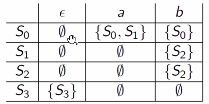
\includegraphics[width=.4\textwidth,keepaspectratio]{tabella}
%     \caption{Tabella}
%     \label{tabella}
% \end{figure}
\begin{table}[H]
	\centering
	\subimport{assets/tables/}{nfa2-table.tex}
    \caption{Tabella della funzione di transizione per l'automa \ref{nfa_grafo_2}}
    \label{nfa2-table}
\end{table} 

Qual è quindi il linguaggio accettato da un automa di questo tipo?\label{linguaggio_definito_da_un_automa} 
Un NFA \(\mathcal{N}\) accetta (o riconosce) una parola \(w\) se e solo se esiste almeno un cammino che parte dallo stato iniziale di \(\mathcal{N}\) ed arriva a \(w\).

Ricorda queste regole di scrittura:
\begin{itemize}
    \item \(\varepsilon \varepsilon\) si scrive \(\varepsilon\);
    \item \(a\varepsilon\) si scrive \(a\);
    \item \(\varepsilon a\) si scrive \(a\).
\end{itemize}

Il linguaggio accettato dall’automa è l’insieme di tutte le parole accettate dall’automa.
Risolviamo, ad esempio, il linguaggio generato dall’automa descritto in figura \ref{nfa_grafo_2}:
\begin{itemize}
    \item \(a\) non appartiene al linguaggio, non esiste un percorso che mi porti ad uno stato finale attraversando un solo arco \(a\);
    \item allo stesso modo non posso trovare la parola \(b\) nel linguaggio;
    \item una parola possibile in questo linguaggio è, ad esempio, \(abb\);
    \item tutte le parole nella forma \(\mathcal{L}(a \mid b)^\ast abb\) sono parte del linguaggio.
\end{itemize}

\noindent Proviamo a determinare il linguaggio dell'NFA descritto in figura \ref{nfa_grafo_3}:

\begin{figure}[htb]
    \centering
    \subimport{assets/figures/}{nfa3_regex-copy.tex}
    \caption{}
    \label{nfa_grafo_3}
\end{figure}

\noindent Il linguaggio accettato da questo NFA è \(\mathcal{L}((a a^* ) \mid ( b b^\ast ))\).

\section{La costruzione di Thompson}
La costruzione di Thompson è una procedura algoritmica che permette di costruire l’automa \(\mathcal{N}\) che genera lo stesso linguaggio denotato da una certa espressione regolare \(r\), ovvero \(\mathcal{L}(\mathcal{N}) = \mathcal{L}(r)\).

\subsection{Definizione}
Anche questa costruzione è espressa in modo induttivo.

\begin{description}
    \item[Base] L'espressione regolare \(r\) è o \(\varepsilon\), oppure un simbolo dell’alfabeto \(a \in \mathcal{A}\); assumiamo di avere sempre un NFA che riconosce \(\mathcal{L}(\varepsilon)\) e uno che riconosce \(\mathcal{L}(a) \; \forall a \in \mathcal{A}\).
    \item[Step] L'espressione regolare \(r\) è una tra le seguenti opzioni: 
    \begin{itemize}[noitemsep]
        \item \(r_1 \mid  r_2 \);
        \item \( r_1 r_2 \); 
        \item \( r_1\) \(^\ast \);
        \item \((r_1)\);
    \end{itemize}
    e, dati gli NFA \(\mathcal{N}_1\) e \(\mathcal{N}_2\) tali che \(\mathcal{L}(\mathcal{N}_1)=\mathcal{L}(r_1)\) e \(\mathcal{L}(\mathcal{N}_2) = \mathcal{L}(r_2)\), dobbiamo definire i vari NFA per le quattro operazioni \(r_1 \mid r_2\), \(r_1 r_2\), \(r_1\) \(^\ast\) ed \(r_1\). Le regole per definire questi nuovi NFA sono elencate successivamente.
\end{description}

\noindent A questo punto possiamo fare due osservazioni sulla costruzione di Thompson.

\begin{enumerate}
    \item Ogni passo della costruzione introduce al massimo due nuovi stati, vale a dire che l’NFA generato contiene al massimo \(2k\) stati, dove \(k\) è il numero di simboli e operatori nell’espressione regolare.
    \item In ogni stato intermedio dell’NFA c’è esattamente uno stato finale, e inoltre lo stato iniziale non ha nessun arco entrante e lo stato finale non ha alcun arco uscente. 
\end{enumerate}

\subsection{Spiegazione in dettaglio}
Vediamo ora la rappresentazione grafica di questo algoritmo. Partiamo dai passi base.

\begin{figure}
    \centering
    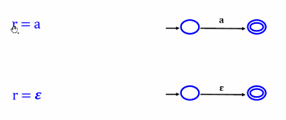
\includegraphics[width=.5\textwidth,keepaspectratio]{Thompson_base}
    \caption{Thompson per il caso base}
    \label{Thompson_base}
\end{figure}

\noindent La spiegazione dell'algoritmo nel caso base è banale, osserviamo invece con più interesse lo step induttivo.

\begin{figure}
    \centering
    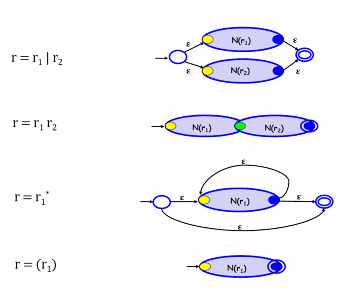
\includegraphics[width=.7\textwidth,keepaspectratio]{Thompson_step}
    \caption{Thompson per lo step induttivo}
    \label{Thompson_step}
\end{figure}
Supponiamo di avere \(\mathcal{N}(r_1)\) e \(\mathcal{N}(r_2)\) descritti come in precedenza, discutiamo le applicazioni di Thompson descritte in in figura \ref{Thompson_step}.

\subsubsection{Alternation}
Guardiamo il primo caso, l'operazione di addizione \(r = r_1 \mid r_2\).\\
Vogliamo creare un automa che accetta parole di \(\mathcal{L}(r_1)\) o anche parole di \(\mathcal{L}(r_2)\).
Abbiamo i due \(\mathcal{N}\), che rappresentano gli stati intermedi; li posizioniamo uno sopra all’altro. Ora possiamo creare uno stato vuoto e usarlo come stato iniziale per entrambi gli \(\mathcal{N}\), e quindi collegarlo a questi ultimi tramite una \(\varepsilon\)-trasformazione; allo stesso modo possiamo creare uno stato finale raggiungibile dai due \(\mathcal{N}\) tramite una \(\varepsilon\)-trasformazione.

\subsubsection{Concatenation}
Guardiamo ora l’operazione di concatenazione \(r = r_1 r_2\).\\
Per la nostra ipotesi induttiva, sappiamo di poter far affidamento sui due automi \(\mathcal{N}(r_1)\) ed \(\mathcal{N}(r_2)\); in questo momento ci viene in aiuto la proprietà della costruzione, che dice che i passi intermedi (i due \(\mathcal{N}\)) hanno esattamente uno stato finale ed uno stato iniziale, senza alcun arco entranto nello stato iniziale e nessun arco uscente dagli stati finali. 
In questo modo possiamo far coincidere lo stato iniziale di \(\mathcal{N}(r_2)\) con lo stato finale di \(\mathcal{N}(r_1)\). 
Di conseguenza, una parola riesce ad arrivare allo stato terminale blu solo se riesce a passare sia da \(\mathcal{N}(r_1)\) che da \(\mathcal{N}(r_2)\).

\subsubsection{Kleene Star}
Guardiamo il caso della Kleene star \(r = r_1^*\).\\
Vogliamo un automa che riconosce o \(\varepsilon\) o tutte le parole che sono composte dalla ripetizione di altre parole appartenenti al linguaggio \(\mathcal{L}(r_1)\).
Posseggo l’automa \(\mathcal{N}(r_1)\), che ha un solo stato iniziale ed un solo stato finale; aggiungo due stati che serviranno come nuovo stato iniziale e nuovo stato finale.
Siccome voglio poter avere \(\varepsilon\) come parola possibile, introduco un nuovo arco \(\varepsilon\) che collega il nuovo stato iniziale al nuovo stato finale, quindi implemento la ripetizione con degli altri archi \(\varepsilon\) come in figura; la spiegazione è abbastanza banale.

\subsubsection{Parentheses}
Guardiamo il caso della parentesizzazione \(r = ( r_1 )\), il quale risulta estremamente banale, così tanto che in realtà non lo guardiamo davvero scherzone lol.

Questo è il modo di utilizzare il processo di Thompson per costruire automi complessi, ci renderemo conto più avanti di quante \(\varepsilon\) questo ci costringe ad utilizzare e di cosa questo comporti.

\subsection{Applicazione di Thompson}
Presentiamo ora un esempio particolare per assimilare meglio questa costruzione. Analizziamo il seguente linguaggio:

\begin{equation}
    r = (a \mid b)^\ast abb
\end{equation}

\noindent Ci sono quindi due espressioni che compaiono in questo esempio: \(a = r_1\) e \(b = r_2\).
In primis applichiamo la regola di base (\ref{Thompson_base}).

\begin{figure}
    \centering
    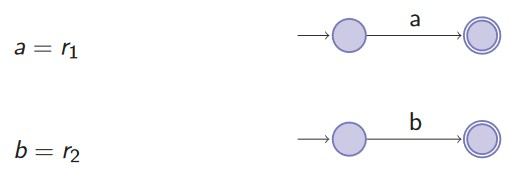
\includegraphics[width=.7\textwidth,keepaspectratio]{esempio_Thompson_0}
    \caption{Applicazione del passo base della costruzione di Thompson}
    \label{esempio_Thompson_0}
\end{figure}

Concentriamoci ora sulla prima espressione, \( a \mid b = r_1 \mid r_2 = r_3\); applichiamo la costruzione di Thompson per l’alternanza ai due automi per \(r_1\) e \(r_2\), otteniamo quindi l’automa per \(r_3\).

\begin{figure}
    \centering
    \subimport{assets/figures/}{thompson1_alternanza.tex}
    \caption{Applicazione della costruzione per l'alternanza}
    \label{esempio_Thompson_1}
\end{figure}

La procedura è rappresentata in figura \ref{esempio_Thompson_1} ed è qui brevemente descritta: prendiamo i due automi per \(r_1\) ed \(r_2\), li mettiamo uno sopra l’altro e generiamo due stati (nodo \(1\) e nodo \(6\)); il nodo \(1\) sarà collegato tramite archi \(\varepsilon\) agli stati iniziali di entrambi gli automi, e simmetricamente il nodo \(6\) verrà collegato tramite archi \(\varepsilon\) agli stati finali dei due automi.

Il prossimo passaggio è la traduzione dell'operatore di parentesi, il che è banale, quindi ne riportiamo solo una formulazione nel linguaggio delle espressioni regolari:

\begin{equation*}
    (a \mid b)=(r_3)=r_4
\end{equation*}

\noindent Ora dobbiamo rappresentare la seguente espressione:

\begin{equation*}
    (a\mid b)^\ast = r_4^\ast = r_5
\end{equation*}

\noindent Quindi applichiamo la costruzione di Thompson per la Kleene star all’automa per \(r_4\), ottenendo quindi l’automa per \(r_5\).

\begin{figure}
    \centering
    \subimport{assets/figures/}{thompson2_kleeny.tex}
    \caption{Applicazione della costruzione per la Kleene star}
    \label{esempio_Thompson_2}
\end{figure}

\noindent Continuando con la scansione dell’espressione regolare dobbiamo riscrivere la seguente:

\begin{equation}
    (a \mid b)^\ast a = r_5 r_1 = r_6
\end{equation}

\noindent Applichiamo quindi la costruzione di Thompson per la concatenazione.

\begin{figure}
    \centering
    \subimport{assets/figures/}{thompson3_conc.tex}
    \caption{Applicazione della costruzione per la concatenazione}
    \label{esempio_Thompson_3}
\end{figure}

\noindent Dobbiamo infine riapplicare il passo della concatenazione per le due \(b\) mancanti.

\begin{figure}
    \centering
    \subimport{assets/figures/}{thompson4_conc.tex}
    \caption{Applicazione della costruzione per la concatenazione (II)}
    \label{esempio_Thompson_4}
\end{figure}

Possiamo notare come il risultato cui giungiamo sia pieno di \(\varepsilon\); la costruzione di Thompson ci dà sicuramente un risultato esatto, ma non è detto che sia il risultato migliore, anzi; abbiamo già visto in passato un automa che riconosce lo stesso linguaggio di questo, e quell'automa era più semplice ed elegante (vedi \ref{nfa_grafo_2}).

Notiamo che comunque l’algoritmo di Thompson garantisce dei limiti superiori sulla complessità dell’automa che genera: ad ogni passo si aggiungono al massimo \(2\) nuovi nodi.
La lunghezza dell’automa finale infatti è limitata da \(2n\), con \(n\) che rappresenta il numero di simboli nell’espressione regolare, dove con simboli si intende sia simboli del vocabolario che operatori.

Anche il numero di archi è limitato in quanto per ogni passaggio si aggiungono al massimo \(4\) archi.

\section{Il processo di simulazione dell’automa}
Le nostre conoscenze attuali ci permettono di costruire un automa per una certa espressione regolare, ma come si fa a decidere se una certa parola \(w\) fa parte del linguaggio di un dato automa \(\mathcal{N}\)? Si utilizza una procedura detta \emph{simulazione dell’automa}.

Abbiamo già definito in \ref{linguaggio_definito_da_un_automa} come viene deciso se una parola fa parte del linguaggio riconosciuto dall’automa; prendiamo ora ad esempio \(w = bbb\) e l’automa presentato in figura \ref{automa_secondo_esempio}, e presentiamo la procedura di simualzione di un automa.

\begin{figure}
    \centering
    \subimport{assets/figures/}{nfa4_simulazione.tex}
    \caption{Esempio di automa}
    \label{automa_secondo_esempio}
\end{figure}

Se dovessimo fare “a occhio”, questo caso sarebbe molto semplice da risolvere: si parte dallo stato \(S_0\) e si va in un altro stato tramite o archi \(\varepsilon\) o tramite archi \(b\); una volta che raggiungo uno stato con un arco \(b\) elimino il primo carattere della parola e procedo con il secondo, cerco archi con \(\varepsilon\) o con il secondo carattere e così via.
La parola appartiene al linguaggio riconosciuto dall’automa se consumo l’ultimo carattere della parola in uno stato finale.

Noi però stiamo cercando un algoritmo formale che faccia queste operazioni, e che le faccia senza necessità di backtrack per tornare indietro se un percorso si rivela errato, operazione altamente costosa.
Cosa possiamo fare per velocizzare il processo?

Vediamo che leggere \(bbb\) da \(S_0\) è uguale a leggerlo da uno qualunque tra gli stati \(\{S_0, S_1, S_3, S_5\}\), perché arrivo a questi stati solo tramite archi \(\varepsilon\); non potremmo quindi semplificare tutti questi in un solo nodo?

La risposta è sì, possiamo farlo! Per vedere in che modo dobbiamo prima introdurre il concetto di \(\varepsilon\)-chiusura.


\subsection{\(\varepsilon\)-chiusura di un automa}
Sia \((S, \mathcal{A}, \textrm{move}_n, s_0, F)\) un NFA, sia \(t\) uno stato in \(S\) e \(T\) un sottoinsieme di \(S\).

Definiamo \(\varepsilon\)-chiusura\((\{t\})\) l’insieme di stati in \(S\) che sono raggiungibili da \(t\) tramite zero o più \(\varepsilon\)-transizioni (nota che \(t\) è sempre in questo insieme).

Definiamo \(\varepsilon\)-chiusura\((T)\) nel seguente modo:
\begin{equation}
    \varepsilon \textrm{-chiusura}(T) = \bigcup_{t \in T} \;\varepsilon\textrm{-chiusura}(\{t\})
\end{equation} 

\subsubsection{Calcolo della \(\varepsilon\)-chiusura}
Per calcolare la \(\varepsilon\)-chiusura di un nodo di un automa useremo queste strutture:

\begin{enumerate}
    \item Uno stack;
    \item Un array booleano “alreadyOn” che ci serve per segnalare se uno stato \(t\) è già sulla pila o meno (la sua lunghezza è \(|S|\));
    \item Un array bidimensionale per ricordare \(\textrm{move}_n\). Ogni entry \((t,x)\) è una lista linkata contenente tutti gli stati che sono raggiungibili con un \(x\)-transizione da \(t\).
\end{enumerate}

Ora che sappiamo quali sono le strutture dati che andremo ad utilizzare, studiamo la fase di inizializzazione: 

\begin{itemize}
    \item all’inizio dei tempi non c’è niente sulla pila, poi inseriamo \(t\) e lo segnaliamo su alreadyOn;
    \item a questo punto estraiamo dalla cima dello stak, prendiamo il nodo estratto \(e\) e cerchiamo tutti i nodi che da \(e\) si raggiugono tramite un \(\varepsilon\)-arco; inseriamo tutti questi nello stak (se non sono già presenti) e ne segnaliamo l'inserimento settando il loro flag su alreadyOn.
\end{itemize}

Continuiamo così finché lo stak non si svuota. L'algoritmo appena descritto si può trovare in figura \ref{algoritmo_epsilon_chiusura}.

% \begin{figure}[H]
%     \centering
%     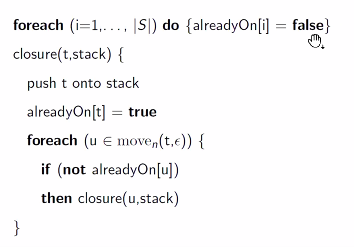
\includegraphics[width=.6\textwidth,keepaspectratio]{algoritmo_epsilon_chiusura}
%     \caption{Algoritmo per il calcolo della \(\varepsilon\)-chiusura\((\{t\})\)}
%     \label{algoritmo_epsilon_chiusura}
% \end{figure}

% \begin{algorithm}[H]
% 	\centering
	\subimport{assets/pseudocode/}{ec-wrapper.tex}
	\subimport{assets/pseudocode/}{ec-computation.tex}\label{algoritmo_epsilon_chiusura}
	% \caption{Esempio di parse tree}
% \end{algorithm}

Ora che abbiamo l'arma della \(\varepsilon\)-chiusura possiamo procedere con l'algoritmo per la verifica dell'appartenenza di una parola \(w\) al linguaggio riconosciuto da un automa, ovvero l'algoritmo di simulazione (figura \ref{algoritmo_simulazione_nfa}).

% \begin{figure}
%     \centering
%     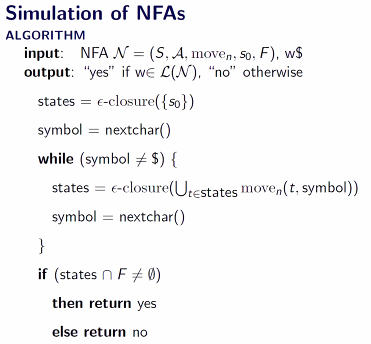
\includegraphics[width=.6\textwidth,keepaspectratio]{algoritmo_simulazione_nfa}
%     \caption{Algoritmo di simulazione per un automa}
%     \label{algoritmo_simulazione_nfa}
% \end{figure}
\subimport{assets/pseudocode/}{nfa-simulation.tex}\label{algoritmo_simulazione_nfa}

Dove \texttt{\$} è l’end-marker per la parola \(w\) (alcuni testi usano la “gratella” invece che \texttt{\$}).
Il funzionamento dell'algoritmo è questo: calcoliamo la \(\varepsilon\)-chiusura di \(s_0\) e la aggiungiamo all'insieme \texttt{states}; prendiamo il primo simbolo nella parola e poi entriamo nel ciclo che compone il corpo della procedura.

In questo corpo si utilizza la \(\varepsilon\)-chiusura per salvare in \texttt{states} la \(\varepsilon\)-chiusura di tutti gli stati che posso raggiungere tramite una \texttt{symbol}-transizione (una transizione marcata con \texttt{symbol}); una volta trovati questi nodi passo \texttt{symbol} prende il valore del prossimo carattere di \(w\).

Una volta che \texttt{symbol} prende il valore di \texttt{\$}, mi fermo e controllo il contenuto di \texttt{states}.

Se \(\textrm{\texttt{states}} \; \cap \; F \neq \Phi\), allora significa che esiste uno stato in \texttt{states} che è anche uno stato finale dell'automa e quindi abbiamo trovato un percorso che riconosce la parola \(w\) e termina in uno stato finale (ammissibile). Ottimo, abbiamo appena dimostrato che \(w\) appartiene al linguaggio riconosciuto dall'automa.

Se invece la condizione precedente non è verificata, allora si è avverato uno dei seguenti casi (o anche entrambi): o non esistono percorsi che riconoscono \(w\), o non esistono percorsi che riconoscono \(w\) e terminano in uno stato finale.

\subsection{Esempi di simulazione}
Applichiamo ora, come esempio, l'algoritmo di simulazione di un NFA dato, verificando se accetta la parola \(w  = ababb\). Lo svolgimento è rappresentato nella tabella \ref{es-sim-1-tbl}.

\begin{figure}
    \centering
    \subimport{assets/figures/}{thompson4_conc.tex}
    \caption{Esempio di simulazione}
    \label{es-sim-1}
\end{figure}
% \begin{figure}
%     \centering
%     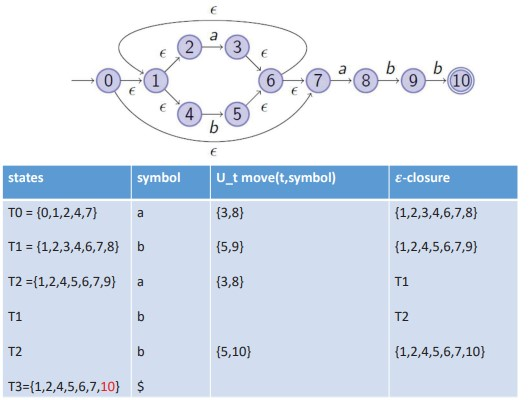
\includegraphics[width=.6\textwidth,keepaspectratio]{simulazione_es_1}
%     \caption{Esempio di applicazione dell'algoritmo di simulazione}
%     \label{simulazione_es_1}
% \end{figure}

\begin{table}[H]
	\centering
	\subimport{assets/tables/}{simulazione-nfa-ex1.tex}
    \caption{Tabella risolutiva della simulazione sull'automa \ref{es-sim-1}}
    \label{es-sim-1-tbl}
\end{table} 

\noindent In seguito una breve descrizione della rappresentazione dell'algoritmo.

Inizializziamo la variabile \texttt{states} a \(T0\) inserendo la \(\varepsilon\)-chiusura di \(0\); poi estraiamo il simbolo da aggiungere (il primo simbolo di \(w\)) che è \(a\).

Ora devo comporre l’insieme di stati che posso raggiungere da \texttt{states} con una \(a\)-transizione, e questo insieme è \(\{3, 8\}\). 

Di questo insieme l’algoritmo dice che devo calcolare la \(\varepsilon\)-chiusura, che corrisponde all’insieme nell’ultima colonna della prima riga; questo è il mio nuovo insieme di stati \(T1\) da cui partirò nello step successivo.

Nel secondo step il simbolo che devo aggiungere è la seconda lettera di \(w\), ovvero \(b\), quindi vado a cercare quei nodi che posso raggiungere da \(T1\) con una \(b\)-transizione; questi nodi sono \(\{5,9\}\), e una volta che li ho trovati ne calcolo la \(\varepsilon\)-chiusura, che compone \(T2\) e via così.

Continuo così finché non finisco i simboli; a quel punto devo verificare se esiste nel mio insieme \(states\) uno stato finale. In questo caso è presente (\(10\)), e quindi la parola \(w\) appartiene al linguaggio riconosciuto dall’automa raffigurato.


\subsection{Nota sulla \(\varepsilon\)-chiusura}
\begin{theorem}
    Sia \((S, \mathcal{A}, \textrm{move}_n, s_0, F)\) un NFA e sia \(M \subseteq S\).
    
    Allora la \(\varepsilon\)-chiusura\((M)\) è il più piccolo insieme \(X \subseteq S\) tale che \(X\) è una soluzione alla seguene equazione:
    \begin{equation}
        X = M \cup \{ N’ \mid N \in X \land N’ \in \textrm{move}_n (N,\varepsilon)\}
        \label{eps-closure-set-eq}
    \end{equation}
\end{theorem}

\noindent Nota che diciamo il più piccolo insieme per evitare di proseguire in loop infiniti come quello rappresentato in figura \ref{nfa_ciclico}.

\begin{figure}
    \centering
    \subimport{assets/figures/}{nfa5_e-closure.tex}
    \caption{Se non scegliessimo il più piccolo \(X\) potremmo incorrere in cicli infiniti.}
    \label{nfa_ciclico}
\end{figure}

Osserviamo con attenzione la formula appena descritta: \(X\) è \(M\) stesso, unito anche a tutti gli stati \(N’\) raggiungibili da \(N\) tramite una \(\varepsilon\)-transizione, dove \(N\) è uno stato qualsiasi in \(M\).

Balza subito all'occhio come la formula per definire \(X\) dipenda da \(X\) stessa; per questo motivo non dovremmo poterla calcolare, giusto? 
Sbagliato! In informatica possiamo risolvere queste equazioni date certe caratteristiche, ed è qui che giunge in nostro aiuto il teorema del punto fisso. 


\subsection{Teorema del punto fisso}
L'equazione \ref{eps-closure-set-eq} vista poco fa è un'istanza di una più generale equazione su insiemi, della forma \(X = f(X)\), sulla quale possediamo un risultato importante.


Sia \(f 2^D \to 2^D\) per qualche insieme finito \(D\) e sia inoltre \( f \) monotona, vale a dire
\begin{equation*}
    X \subseteq Y \implies f(X) \subseteq f(Y)
\end{equation*}
allora esiste una precisa tecnica, basata su approssimanti successivi, per risolvere l'equazione \(X = f(X)\). Adesso vediamo meglio il teorema cui fa riferimento.

\begin{theorem}
    Sia \(S\) un insieme finito e sia \(f 2^S \to 2^S\) una funzione monotona; allora \(\exists m \in \mathbb{N}\) tale che esiste un'unica soluzione minima all'equazione \(X = f(X)\), e questa soluzione è \(f^m(\varnothing)\).
\end{theorem}

\begin{proof}
    I due asserti andranno dimostrati separatamente; come prima cosa, vogliamo dimostrare che \(\exists m \in \mathbb{N}\) tale che \(f^m(\varnothing)\) è soluzione per \(X = f(X)\); prima di procedere è inoltre consigliabile avere ben presente la forma della funzione \(f(X)\) si veda \ref{eps-closure-set-eq}.

    Per definizione stessa di \(f(X)\), possiamo subito dire che \(\varnothing \subseteq f(\varnothing)\) e, poiché \(f(X)\) è monotona, possiamo subito dire anche che \(\varnothing \subseteq f^2(\varnothing)\). Quindi, per il principio di induzione, possiamo affermare senza timore di smentita che \(f^i(\varnothing) \subseteq f^{i + 1}(\varnothing), \forall i \in \mathbb{N} \). A questo punto, possiamo quindi dire di avere una sorta di catena di relazioni tra insiemi:
    \begin{equation*}
        f(\varnothing) \subseteq f^2{\varnothing} \subseteq f^3(\varnothing) \subseteq \ldots
    \end{equation*}
    Questa successione è infinita, ma \(2^S\) è definito come finito, per cui gli insiemi della successione non possono essere tutti diversi l'uno dall'altro! Arriveremo infatti, a un certo punto, a non riuscire più a osservare cambiamenti a successive applicazioni di \(f(X)\); formalmente, troveremo un qualche indice \(m\) tale che:
    \begin{equation*}
        f^m(\varnothing) = f^{m + 1} (\varnothing) = f(f^m(\varnothing))
    \end{equation*}
    Si dice che siamo arrivate al punto di \emph{saturazione}; in questa situazione, possiamo dire che \(f^m(\varnothing)\) è una soluzione per \(X = f(X)\).

    Andiamo adesso a dimostrare che \(f^m(\varnothing)\) è l'unica soluzione minima.\\
    Per assurdo, supponiamo che esista un'altra soluzione \(A\) per \(X = f(X)\); quindi, per ipotesi, deve valere \(A = f(A)\), e quindi dovremo avere che \(A = f(A) = f^2(A) = \ldots = f^m(A)\). Sappiamo anche che \(f^m(\varnothing) \subseteq f^m(A)\), poiché naturalmente l'insieme vuoto è compreso in qualsiasi insieme (\(\varnothing \subseteq A\)) e la funzione \(f\) è monotona. Ma allora possiamo mettere assieme le due precedenti osservazioni e affermare quindi che \(f^m(\varnothing) \subseteq A\), poiché \(f^m(\varnothing) \subseteq f^m(A)\) e \(A = f^m(A)\). Per cui \(f^m(\varnothing)\) è una soluzione unica, ed è anche l'unica minima. 

\end{proof}

Nonostante a prima vista il significato o anche la stessa utilità di questo risultato possa non essere del tutto chiaro, vale la pena di vederlo almeno una volta, poiché tutta la teoria che riguarda la semantica dei linguaggi di programmazione è basata su questo teorema. 

Ad esempio, l'esecuzione di una funzione fattoriale: essa è costituita di una sequenza di costrutti \texttt{while} tali da produrre il risultato per l'input desiderato; ogni iterazione del \texttt{while} calcola un'approssimante del risultato, che viene quindi ricostruito piano piano. È chiaro che in questo esempio non stiamo aggiungendo insiemi ma valori interi, però è utile pensarlo per avere quantomeno un'idea intuitiva di come il teorema del punto fisso sia applicato alla teoria della semantica dei linguaggi di programmazione.

\section{Considerazioni sull'efficienza degli algoritmi sugli NFA}
All'inizio della trattazione sugli automi non deterministici, il nostro obiettivo era riconoscere un linguaggio regolare attraverso degli automi a stati finiti; in particolare, abbiamo detto che l'analisi lessicale utilizzerà le espressioni regolari per identificare i vari elementi del programma scritto. Dalle espressioni regolari vogliamo quindi avere degli strumenti che ci permettono di prendere come input il testo edlprogramma e ottenere in output un flusso di token, che saranno i terminali della grammatica che ha generato il nostro linguaggio.

Ci chiediamo quale sia la complessità degli algoritmi che abbiamo visto per risolvere questa richiesta, anche in vista del momento in cui ci troveremo a scegliere quale tipo di automa scegliere (NFA o DFA) per assolvere diverse tipologie di compiti.

\paragraph{Sunto delle procedure viste}
Data una parola e data un'espressione regolare che denota quello stesso linguaggio, si dica se la parola appartiene a quel particolare linguaggio oppure no. Gli algoritmi che abbiamo visto ci consento di rispondere a questa richiesta applicando le seguenti operazioni:
\begin{itemize}
    \item consideriamo un'espressione regolare \(r\);
    \item applichiamo la costruzione di Thompson e generiamo un NFA che riconosce esattamente il linguaggio denotato da \(r\);
    \item lancia l'algoritmo di simulazione per l'NFA generato.
\end{itemize}
Andiamo quindi ad analizzare la complessità di queste procedure.

\subsection{Complessità della costruzione di Thompson}
Consideriamo la  complessità di generazione di un NFA con \(n\) nodi e \(m\) archi; conoscendo le quattro operazioni, sappiamo che, per ogni passo, aggiungeremo al massimo \(2\) nodi e \(4\) archi (dalla Kleene star, l'operazione più costosa), per cui avremo che \(n \le 2|r|\) e \(m \le 4|r|\), per cui abbiammo che la somma \(n + m\) è dell'ordine della dimensione dell'espressione regolare (\(\mathcal{O}(|r|)\)) e, poiché avremo in totale \(|r|\) passi, ciascuno dei quali eseguibile in tempo costante, possiamo felicemente comcludere che \(T(\textrm{Thompson}(r)) = \mathcal{O}(|r|)\).

\subsection{Complessità del calcolo della \(\varepsilon\)-chiusura}
Prima di analizzare il costo della simulazione, dobbiamo analizzare il costo della \(\varepsilon\)-chiusura. Teniamo in mente il listato di codice che ne descrive l'algoritmo:

% \begin{figure}
%     \centering
%     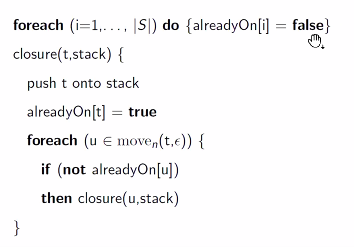
\includegraphics[width=.6\textwidth,keepaspectratio]{algoritmo_epsilon_chiusura}
%     \caption{Algoritmo per il calcolo della \(\varepsilon\)-chiusura\((\{t\})\)}
%     \label{algoritmo_epsilon_chiusura}
% \end{figure}
\subimport{assets/pseudocode/}{ec-wrapper.tex}
\subimport{assets/pseudocode/}{ec-computation.tex}

\noindent Evidenziamo che le strutture usate sono uno: stack (per contenere gli elementi non ancora incontrati), un vettore booleano (per tenere traccia dei visitati), e \(
\textrm{move}_n\), al solito un vettore bidimensionale di puntatori liste linkate, ciascuna contente tutti gli stati raggiungibile a partire da uno stato \(t\) e un simbolo \(x\).

In sunto, la procedura si compone dei seguenti quattro passi:

\begin{enumerate}
    \item inserimento del nodo \(t\) nello stack;
    \item imposta \texttt{alreadyOn[t] = true};
    \item trova un successivo nodo \(u \in \textrm{move}_n(t, \varepsilon)\);
    \item verifica se è già stato visitato con \texttt{alreadyOn[u]}.
\end{enumerate}

\noindent Ognuna di queste operazioni opera in tempo costante, ci chiediamo quindi quante volte venga ripetuto ognuna di queste.

Osserviamo che le prime due operazioni vengono ripetute a ogni chiamata della procedura, e mai più di una volta per ogni nodo, dal momento che il vettore \texttt{alreadyOn} non ci permetterà di richiamare la funzione se lanciato su un nodo già settato a \texttt{true}, e non capita mai che qualche bit venga reinizializzato a false. Per cui, il costo delle prime due operazioni è \(\mathcal{O}(n)\).

La terza e la quarta oeprazione vengono eseguite per ogni nodo raggiungibile con una \(\varepsilon\)-transizione, per cui possiamo immaginare un caso pessimo in cui ogni stato possiede almeno una \(\varepsilon\)-transizione; nel caso peggiore, quindi, andremo a visitare ogni arco del grafo (\(\mathcal{O}(m)\)).

Complessivamente, il costo della procedura è \(\mathcal{O}(n + m)\).

\subsection{Complessità della simulazione di NFA}
Adesso possiamo affrontare il problema dello studio della complessità della simulazione di NFA. Anche qui, teniamo presente il codice:

% \begin{figure}
%     \centering
%     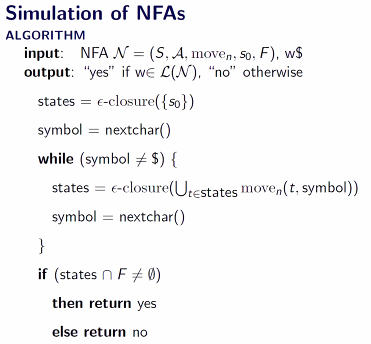
\includegraphics[width=.6\textwidth,keepaspectratio]{algoritmo_simulazione_nfa}
%     \caption{Algoritmo di simulazione per un automa}
%     \label{algoritmo_simulazione_nfa}
% \end{figure}
\subimport{assets/pseudocode/}{nfa-simulation.tex}

\noindent Anche qui, un veloce recapdelle strutture dati utilizzate. Innanzitutto si tenga presente che, per tenere traccia della variabile \texttt{states}, utilizzeremo ben due stacks:

\begin{itemize}
    \item il primo (\texttt{currentStack}) è nel right value della riga \(4\) e viene utilizzato per conservare il contenuto del vettore \texttt{states} durante l'attuale iterazione dell'algoritmo;
    \item il secondo (\texttt{nextStack}) è invece  nel left value e verrà aggiornato durante la attuale iterazione.
\end{itemize}

\noindent Abbiamo anche il nostro vettore \texttt{alreadyOn} di dimensione \(|S|\) e, naturalmente, il vettore bidimensionale per conservare \(\textrm{move}_2\).

Ci rendiamo conto che il ciclo \texttt{while} domina la complessità, soprattutto perché al suo interno avviene una chiamata di \(\varepsilon\)-chiusura, completata dall'estrazione di tutti gli elementi da \texttt{nextStack} e il loro inserimento in \texttt{currentStack}, oltre alla reinizializzazione di \texttt{alreadyOn}.

% \begin{figure}
%     \centering
%     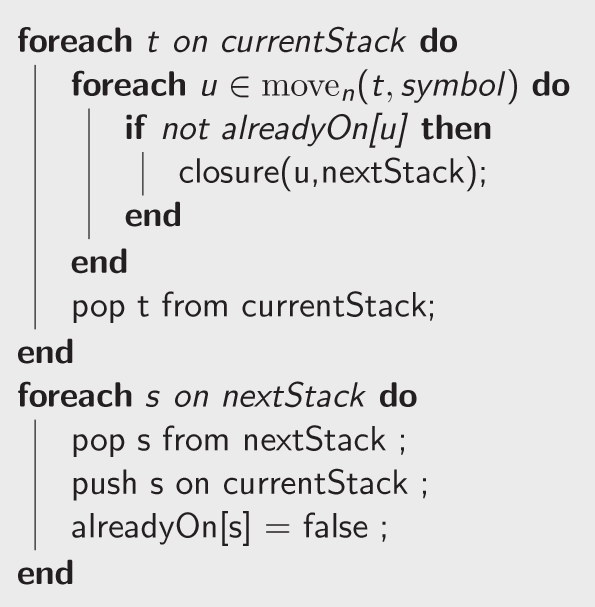
\includegraphics[width=.6\textwidth,keepaspectratio]{algoritmo_simulazione_nfa_2}
%     \caption{Dettaglio di algoritmo di simulazione per un automa}
%     \label{algoritmo_simulazione_nfa_2}
% \end{figure}
\subimport{assets/pseudocode/}{nfa-sim-line4.tex}

All'interno di ogni \texttt{while}, quindi, abbiamo uno swap degli stack, che costa \(\mathcal{O}(n)\), poiché è limitato dal numero di nodi dell'NFA; inoltre, ogni stato può essere inserito solo una volta nella pila nel secondo \texttt{foreach}; quindi, ogni ciclo del \texttt{while} costa \(\mathcal{O}(n + m)\). Questo ciclo verrà lanciato per ogni elemento della parola \(w\) analizzate, pertanto il costo complessivo della simulazione è \(\mathcal{O}(|w|(n + m))\); dal momento che il nostro NFA è stato generato da un'esecuzione di costruzione di Thompson, avremo anche che \(n + m = \mathcal{O}(|r|)\), per cui possiamo concludere che il costo  dell'intera procedura di simulazione è dell'ordine di \(\mathcal{O}(|w||r|)\).

Il costo è sicuramente più basso di quello che avrei facendo del backtrack, dal momento che si parla comunque di un modello non deterministico. 

\section{Automa a stati finiti deterministico}
Possiamo pensare di utilizzare queste strutture per decidere se accettare delle parole e determinare se appartiene a un linguaggio denotate da un'espressione regolare.

Introdunciamoli per differenza rispetto agli NFA. Si tenga  amente la definizione di NFA:

\begin{gather*}
    \mathcal{N} := (S, \mathcal{A}, \textrm{move}_n, s_0, F), \textrm{ dove } \\
    \textrm{move}_n : S \times (\mathcal{A} \cup \{\varepsilon\}) \to 2^S
\end{gather*}

Si noti la funzione di transizione, che opera con uno stato e un simbolo dell'alfabeto, unito a \(\varepsilon\), e proprio quest'ultima apporta l'elemento di indeterminazione; inoltre, un qualunque nodo di un grafo ha tendenzialmente più archi uscenti identificati dal medesimo simbolo.

Un automa a stati finiti deterministici è invece definito come segue:

\begin{gather*}
    \mathcal{D} := (S, \mathcal{A}, \textrm{move}_d, s_0, F), \textrm{ dove } \\
    \textrm{move}_d : S \times \mathcal{A} \to S
\end{gather*}

Balza subito la differente formulazione della funzione di transizione, il cui dominio esclude la possibilità di compiere \(\varepsilon\)-transizioni. Inoltre, quest'ultima ha due modi di presentarsi: totale o parziale, e il possesso dell'una o dell'altra qualificazione inficerà la scelta delle procedure da applicare.

Evidenziamo le caratteristiche dei DFA:

\begin{itemize}
    \item non presentano \(\varepsilon\)-transizioni (ma c'è un cavillo di cui ci occuperemo più avanti);
    \item se \(\textrm{move}_d\) è \emph{totale}, allora per ogni stato c'è \textbf{esattamente} una \(a\)-transizione \(\forall a \in \mathcal{A}\);
    \item se \(\textrm{move}_d\) è \emph{parziale}, allora per ogni stato c'è \textrm{almeno} una \(a\)-transizione \(\forall a \in \mathcal{A}\); in altre parole, per alcune coppie del dominio la funzione non è definita.
\end{itemize}

% TODO prova ad usare il pacchetto subfigure
\begin{figure}[H]
    \begin{minipage}[b]{0.4\textwidth}
        \centering
        \subimport{assets/figures/}{dfa_total_transition.tex}
        \subcaption{Esempio di funzione di transizione totale}
    \end{minipage}
    \hfill
    \begin{minipage}[b]{0.4\textwidth}
        \centering
        \subimport{assets/figures/}{dfa_partial_transition.tex}
        \subcaption{Esempio di funzione di transizione parziale}
    \end{minipage}
    \caption{Funzioni di transizione dei DFA}
\end{figure}

\subsection{Linguaggi rionosciuti dai DFA}
Prendiamoci un certo DFA \(\mathcal{D} = (S, \mathcal{A}, \textrm{move}_d, s_0, F)\); il linguaggio \(\mathcal{L(D)}\) da lui riconosciuto è l'insieme di parole \(w\) tale che:

\begin{itemize}
    \item o esiste un cammino, che chiamiamo qui \(w = a_1, \ldots, a_k\), con \(k \ge 1\), che vada dallo stato iniziale \(s_0\) a un qualche stato finale in \(F\);
    \item oppure vale che \(s_0 \land w \in F\); per l'appunto, quello in cui lo stato di partenza è uno stato finale è l'unico caso in cui un DFA possiede la parola vuota.
\end{itemize}

\subsection{Simulazione di un DFA con transizione totale}
In questo caso abbiamo la certezza che, per ogni  simbolo che leggiamo, ci sia un qualche arco che lo colleghi a uno stato successivo nel grafo, e questo semplifica di molto la procedura per determinare se una certa parola \(w\) appartenza o meno al linguaggio del nostro DFA.

Per l'appunto, è sufficiente partire dallo stato iniziale \(s_0\) e seguire il cammino dato dagli elementi di \(w\); se terminiamo in un qualche stato finale in \(F\), allora \(w\) appartiene al linguaggio, altrimenti no; la complessità, pertanto, è \(\mathcal{O}(|w|)\).

\subsection{Simulazione di un DFA con transizione parziale}
Poiché qui abbiamo una funzione di transizione totale, dobbiamo considerare la possibilità di arrivare a uno stato in cui non non possiamo più proseguire. 

Iniziamo comunque dallo stato iniziale e, di nuovo, seguiamo il cammino dato dallo spelling della parola \(w = a_1, a_2, \ldots, a_k\); se sto leggendo un qualche simbolo per cui non c'è una transizione "etichettato" da quel simbolo, allora posso direttamente ritornare una risposta negativa; se invece riesco a leggere tutta la parola e a raggiungere uno stato finale, posso rispondere affermativamente.

\subsection{Funzioni di transizioni a confronto}
Dato un DFA \(\mathcal{D}\) con funzione di transizione parziale, ho un modo per definire un DFA \(\mathcal{D}'\) che abbia funzione di transizione totale e che riconosca esattamente lo stesso linguaggio (\(\mathcal{L(D) = \mathcal{L}(\mathcal{D}')}\))?

Posso farlo con l'uso di un \emph{sink} (anche detto dead state, o in italiano stato trappola). In sostanza vado a creare un nuovo stato che aggiungo subito agli altri stati di \(\mathcal{D}\), e questo stato sarà la destinazione di tutte le transizioni non definite dalla funzione di transizione; infine, per ogni simbolo dell'alfabeto, aggiungo al sink un \emph{self loop} su quel simbolo.

In questo modo, quando vado a trovarmi in quelle situazioni in cui non potevo più proseguire, posso invece proseguire e andare nel sink; in questo modo potrò comunque continuare, esaurire la parola in uno stato non terminale e quindi tornare un risultato coerente con il linguaggio considerato.

In generale si preferisce lavorare con DFA con funzione di transizione parziale, e ancora più in generale con automi che abbiamo il minor numero di stati (nodi e archi) possibile; tuttavia, l'algoritmo di minimizzazione (vedremo più avanti), che usiamo per "ridurre al minimo" il suo numero di archi e nodi, non funziona con DFA privi di funzione di transizione totale. Il motivo sta nel fatto che questa procedura lavora sulla funzione inversa di \(\textrm{move}_d\), che chiaramente non è definita se la funzione non è totale.


\section{Traduzione da NFA a DFA}
Abbiamo già discusso in passato di come la simulazione su DFA sia più efficiente che su NFA, quindi ora siamo interessati a risolvere questo problema: dato un qualunque NFA some si può ricavare un DFA che riconosca lo stesso linguaggio?

Un mezzo per raggiungere questo scopo è l’utilizzo di una sorta di meccanismo di \(\varepsilon\)-chiusura permanente (che elimini in modo permanente le \(\varepsilon\)-transizioni), questo meccanismo si chiama Subset Construction.


\subsection{Algoritmo di Subset Costruction}
L’algoritmo di Subset Construction serve per ricavare un DFA dato un certo NFA.

L'idea di base è quella di utilizzare la \(\varepsilon\)-chiusura per mappare sottoinsiemi degli stati del dato NFA (che in seguito chiameremo rozzamente \emph{stati non deterministici}, o \emph{snd}) in stati per il nuovo DFA (che in seguito chiameremo rozzamente \emph{stati deterministici} o \emph{sd}).

Per dare un'idea di come lavora questo algoritmo descriviamone i primi passi.\\
Si individua qual è lo stato iniziale dell'NFA, diciamo \(S_0\), lo si prende come punto di partenza e se ne calcola la \(\varepsilon\)-chiusura \(T\); sarà proprio \(T\) ad essere lo stato iniziale del DFA. Ora dovrebbe essere più chiaro quello che si fa in questo algoritmo: si eliminano tutte le \(\varepsilon\)-transizioni per ottenere un set di transizioni \(\textrm{move}_d\) che contiene solo transizioni "deterministiche".

Un fatto da tenere sempre ben presente è che gli stati del DFA che otteniamo in questo modo sono insiemi di stati dell'NFA di partenza. Il \(T\) appena descritto è un sottoinsieme degli stati dell'NFA di partenza.

Dopo questa piccola introduzione passiamo a visualizzare subito il codice dell'algoritmo di Subset Construction.

%  (figura \ref{algoritmo_subset_construction})
% \begin{figure}
%     \centering
%     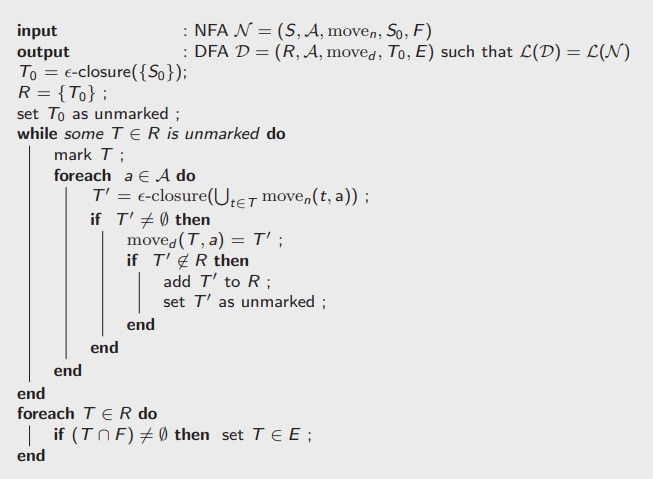
\includegraphics[width=.8\textwidth,keepaspectratio]{subset_construction_algorithm.jpg}
%     \caption{Algoritmo di Subset Construction}
%     \label{algoritmo_subset_construction}
% \end{figure}
\subimport{assets/pseudocode/}{subset-construction.tex} 
\noindent Procediamo quindi ora con una spiegazione discorsiva di questo algoritmo.
\paragraph*{Input}
L'algoritmo prende come input un NFA specificato dalla tupla \(\mathcal{N} := (S, \mathcal{A}, \textrm{move}_n, s_0, F)\)

\paragraph*{Output}
L'algoritmo ritorna come output un DFA specificato dalla tupla \(\mathcal{D} := (R, \mathcal{A}, \textrm{move}_d, s_0, E)\) tale da soddisfare la condizione \(\mathcal{L}(\mathcal{D}) = \mathcal{L}(\mathcal{N})\).

\paragraph*{Introduzione}
Per prima cosa si calcola quello che sarà lo stato iniziale del DFA, ovvero \(T_0\); esso è coinciderà, come già detto in precedenza, con la \(\varepsilon\)-chiusura dello stato iniziale dell'NFA \(S_0\). Una volta calcolato questo \(T_0\),  lo si inserisce nell'insieme \(R\) e lo si segna come unmarked.

\paragraph*{Ciclo while}
Qui inizia il corpo centrale dell'algoritmo: questo ciclo serve per iterare su tutti gli stati che si stanno inserendo mano a mano nell'insieme degli stati del DFA. 

Di fatto, dentro al ciclo si scorrono tutti gli stati in \(R\) e ci si sofferma sugli stati \(T \in R\) segnati come \texttt{unmarked}. Di volta in volta, quando se ne identifica uno, lo si marca, dimodoché che non venga più elaborato in seguito, e si procede con l'elaborazione.

\paragraph*{Foreach interno al ciclo while}
In questa fase si scorrono tutti gli elementi \(a\) dell'alfabeto \(\mathcal{A}\) e si prosegue quindi in questo modo:
\begin{itemize}
    \item si prendono tutti gli stati (snd) raggiungibili dallo stato (sd) \(T\) che soddisfino la seguente condizione \(\cup_{t \in T} \textrm{move}_n(t,a)\), ovvero tutti gli stati in \(S\) raggiungibili tramite una \(a\)-transizione da uno degli stati in \(T\), se ne calcola la \(\varepsilon\)-chiusura e la si salva nella variabile \(T'\);
    \item una volta calcolato \(T'\) si verifica se questo è vuoto, e se lo è si passa alla prossima iterazionde del \texttt{foreach};
    \item altrimenti, si aggiunge all'insieme delle transizioni ("deterministiche") \(\textrm{move}_d\) la transizione \(\textrm{move}_d(T, a) = T'\);
    \item infine, se \(T'\) non è già presente in \(R\) allora ve lo si aggiunge e si segna come unmarked.
\end{itemize}

\paragraph*{Foreach finale}
Questa fase serve per definire quali sono gi stati (sd) finali del nuovo insieme di stati \(R\), ovvero quali sono gli stati finali del DFA \(\mathcal{D}\). Questi stati (ribadiamo, sd) si identificano perché contengono \emph{almeno uno} stato (snd) finale, ovvero uno stato \(T \in R\) è uno stato finale per \(\mathcal{D}\) se \(T \cap F \neq \Phi\).

Arriva però il momento di porsi un'importante domanda: qual è la complessità di questo algoritmo?
Poniamo le basi per affrontare una risposta: supponiamo che l’NFA abbia \(n\) stati ed \(m\) archi, mentre supponiamo che il DFA abbia \(n_d\) stati.
\begin{itemize}
    \item Osserviamo che il ciclo dominante naturalmente è il primo \texttt{while}; quest'ultimmo  è ritpetuto \(n_d\) volte, ma quanto vale \(n_d\)? Questo è un aspetto che affronteremo nel prossimo futuro.
    \item All'interno del \texttt{while} troviamo il nostro caro \texttt{foreach} \(a \in \mathcal{A}\), che viene ripetuto \(|A|\) volte.
    \item L'ultimo fattore di peso rilevante è la chiamata alla funzione di calcolo della \(\varepsilon\)-chiusura, la quale ha costo \(\mathcal{O}(n+m)\).
\end{itemize}
La complessità globale è quindi \( \mathcal{O}(n_d \cdot |A| \cdot (n+m))\).

Ora la domanda si fa più pressante: quanto vale effettivamente \(n_d\)?
Fin massa... possiamo già anticipare che esso è un \(\mathcal{O}(2^n)\). Nonostante questo possa essere oltremodo sconfortante, è opportuno specificare che quella appena vista è la complessità per \emph{creare} il DFA, un'operazione che viene effettuata una tantum solamente in sede di creazione del compilatore; è vero, è una grossa spesa iniziale, ma permette di avere grandi vantaggi in tutti gli utilizzi successivi.

Tuttavia per applicazioni con tempo di vita più limitato spesso non ha senso creare il DFA, poiché non si avrebbe il tempo di compensare la spesa iniziale; è questa la ragione per cui ad esempio \href{https://it.wikipedia.org/wiki/Grep}{grep} utilizza NFA.


\subsection{Esercizi di applicazione della Subset Construction}
\subsubsection*{Esercizio 1}
Dato l'automa a stati finiti non deterministico in figura \ref{es_sc_1}, calcola, tramite l'algoritmo di Subset Construction, un automa a stati finiti deterministico che riconosca lo stesso linguaggio.
\begin{figure}[H]
    \centering
    \subimport{assets/figures/}{subset_constr_1_NFA.tex}
    \caption{Esercizio 1: NFA}
    \label{es_sc_1}
\end{figure}

Il modo più semplice e chiaro per risolvere questo tipo di esercizi è quello di utilizzare una tabella per scrivere i vari passaggi; noi riportiamo qui sotto la soluzione dell'esercizio in tale forma, seguita da un esteso commento della procedura seguita.
\begin{table}[H]
	\centering
	\subimport{assets/tables/}{sol-sc-ex1.tex}
    \caption{Soluzione esercizio 1}
    \label{sol-sc-ex1}
\end{table} 
Lo stato iniziale dell'NFA è \(1\), quindi per calcolare lo iniziale del DFA devo calcolare la \(\varepsilon\)-chiusura di \(1\); questo passaggio è riportato a riga \(1\), colonna \(0\).

Poi entro nel vivo del \texttt{while}: estraggo \(T0\) e devo trovare tutti gli stati raggiungibili da \(T0\) tramite una \(a\)-transizione. In questo modo ottengo lo stato \(3\); di questo insieme di stati (\(\{3\}\)) devo calcolare la \(\varepsilon\)-chiusura, e questa sarà il nuovo insieme \(T1\); aggiungo la transizione \(\textrm{move}_d(T0, a)=\{T1\}\), segno \(T1\) come unmarked e passo avanti.

Adesso devo trovare tutti gli stati raggiungibili da \(T0\) attraverso una \(b\)-transizione. In questo caso ottengo solo lo stato \(5\), e di questo insieme (\(\{5\}\)) calcolo la \(\varepsilon\)-chiusura; questa risulta essere \(\{5\}\). Ho appena trovato \(T2\), lo segno come unmarked e aggiungo la transizione \(\textrm{move}_d(T0, b)=\{T2\}\).

Passo infine ad analizzare lo stato \(T1\). Estraggo \(T1\) da \(R\) e vado a cercare la \(\varepsilon\)-chiusura dei punti di arrivo delle \(a\)-transizioni che partono da \(T1\); trovo che l'unica \(a\)-transizione che, partendo da \(T1\), mi porta allo stato \(3\), e la \(\varepsilon\)-chiusura di \(\{3\}\) mi ritorna esattamente \(T1\). Quindi, quello che sto facendo altro non è che aggiungere la transizione \(\textrm{move}_d(T1, a)=\{T1\}\) al nostro DFA, ma dato che \(T1\) è già marked non lo riaggiungo ad \(R\) e termino qui la mia analisi.

Passo ora alla \(\varepsilon\)-chiusura dei punti di arrivo delle \(b\)-transizioni. Da \(T1\) non parte nessuna \(b\)-transizione, quindi termino qui l'analisi di \(T1\) e passo a \(T2\).
Per \(T2\) compio banalmente le stesse azioni che ho svolto per \(T1\), che quindi non sono qui riportate.

Alla fine della fiera, devo trovare quali sono gli stati finali del nostro automa deterministico, quindi faccio le varie intersezioni (come descritto dall'algoritmo) e segno come stati (deterministici) finali tutti quegli stati (deterministici) che contengono almeno uno stato (non deterministico) che sia esso stesso finale nell'NFA.

Una volta terminata questa operazione abbiamo trovato quindi l’automa a stati finiti deterministico che riconosce lo stesso linguaggio dell’NFA di partenza; possiamo vederne una raffigurazione in figura \ref{sol_sc_1}.
\begin{figure}[H]
    \centering
    \subimport{assets/figures/}{subset_constr_1_DFA.tex}
    \caption{Esercizio 1: DFA}
    \label{sol_sc_1}
\end{figure}


\subsubsection*{Esercizio 2}
Dato l'automa a stati finiti non deterministico in figura \ref{es_sc_2}, calcola tramite l'algoritmo di Subset Construction un automa a stati finiti deterministico che riconosce lo stesso linguaggio.
\begin{figure}[H]
    \centering
    \subimport{assets/figures/}{subset_constr_2_NFA.tex}
    \caption{Esercizio 2: NFA}
    \label{es_sc_2}
\end{figure}
È riportata in seguito la tabella risolutiva per questo esercizio.\\

\begin{table}[H]
	\centering
	\subimport{assets/tables/}{sol-sc-ex2.tex}
    \caption{Soluzione esercizio 2}
    \label{sol-sc-ex2}
\end{table} 

Dato che lo svolgimento dei pass dell'algoritmo non presenta né novità né difficoltà in questo esempio, non è fornita una spiegazione estesa dei passaggi.

A questo punto abbiamo considerato tutti gli stati in \(R\) quindi ora è il momento di determinare quali sono gli stati (deterministici) finali. L’unico stato finale nell'NFA è \(E\), quindi tutti e solo gli stati deterministici che contengono \(E\) sono stati deterministici finali. \(T0\), \(T1\) e \(T2\) sono tutti stati finali. Il DFA risultante si può ammirare in figura \ref{sol_sc_2}.
\begin{figure}[H]
    \centering
    \subimport{assets/figures/}{subset_constr_2_DFA.tex}
    \caption{Esercizio 2: DFA}
    \label{sol_sc_2}
\end{figure}

\subsubsection*{Esercizio 3}
Dato l'automa a stati finiti non deterministico in figura \ref{es_sc_3}, calcola tramite l'algoritmo di Subset Construction un automa a stati finiti deterministico che riconosce lo stesso linguaggio.
\begin{figure}[H]
    \centering
    \subimport{assets/figures/}{thompson4_conc.tex}
    \caption{Esercizio 3: NFA}
    \label{es_sc_3}
\end{figure}
Come per l'esercizio precedente, è riportata in seguito la tabella risolutiva.\\

\begin{table}[H]
	\centering
	\subimport{assets/tables/}{sol-sc-ex3.tex}
    \caption{Soluzione esercizio 3}
    \label{sol-sc-ex3}
\end{table}

Quindi abbiamo ben \(5\) stati per il DFA questa volta! Ora, gli stati finali sono solo quelli che contengono lo stato \(10\) dell'NFA, il che significa che solo \(T4\) è uno stato finale per il DFA ricavato; tale DFA si può vedere in figura \ref{sol_sc_3}.
\begin{figure}[H]
    \centering
    \subimport{assets/figures/}{es1_DFA_minimization.tex}
    \caption{Esercizio 3: DFA}
    \label{sol_sc_3}
\end{figure}

Il lettore attento avrà notato che, a suo tempo, avevamo già visto l'automa non deterministico in figura \ref{es_sc_3}, e in quel momento avevamo già osservato come questo automa riconosca tutte le parole scritte secondo la formulazione \((a \mid b)^* abb\).

Il fatto interessante è che avevamo anche incontrato un altro automa che riconosce lo stesso linguaggio, il quale presentava solo \(4\) stati ed era molto più semplice e compatto di quello che abbiamo appena ricavato. Questo automa è riportato in figura \ref{sol_sc_3_v2} per completezza.

Questo va detto per sottolineare come l'algoritmo di Subset Construction sia un algoritmo che produce \emph{una} soluzione al problema di traduzione DFA \(\to\) NFA, ma non è detto che produca la soluzione \emph{migliore} per questo problema.

\begin{figure}[htb]
    \centering
    \subimport{assets/figures/}{nfa2.tex}
    \caption{Esercizio 3: soluzione alternativa}
    \label{sol_sc_3_v2}
\end{figure}

Da notare che l'automa a stati finiti riportato in figura non è deterministico, ma solo per la presenza di una \(\varepsilon\)-transizione e di due transizioni da \(S_{0}\) col simbolo \(a\)

\section{Minimizzazione di DFA}
Spesso e volentieri non siamo interessati ad un generico DFA \(\mathcal{D}\) che generi un altrettanto generico linguaggio \(\mathcal{L(D)}\), ma desideriamo invece il DFA \(\mathcal{D}'\) minimo, ovvero quello con numero minimo di stati tale che \(\mathcal{L(D)} = \mathcal{L(D')}\). 


Prima di procedere, dobbiamo definire la nozione di \emph{State Equivalence}.

\subsection{Definizione di State Equivalence}

\begin{definition}
    Sia \(\mathcal{D} = (S,\mathcal{A},\textrm{move}_{d},s_{0},F)\) un DFA con funzione di transizione totale. Allora due stati \(s,t \in S\) si dicono equivalenti se e solo se la seguente condizione è verificata:

    \begin{equation}
        \textrm{move}_{d}\!^{*}(s,x) \in F \iff \textrm{move}_{d}\!^{*}(t,x) \in F,  \forall x \in \mathcal{A}^{*} 
    \end{equation}
    
    \noindent dove la funzione multi-passo \(\textrm{move}_{d}\!^{*}\) è definita per induzione sulla lunghezza della stringa considerata nel seguente modo:

    \begin{description}
        \item[Base] \(\textrm{move}_{d}\!^{*}(s,\epsilon)=s\) 
        \item[Step] \(\textrm{move}_{d}\!^{*}(s,wa)= \textrm{move}_{d}(\textrm{move}_{d}\!^{*}(s,w),a)\)
    \end{description}    
\end{definition}

L'idea generale su cui si basa l'algoritmo di minimizzazione qui proposto è che alcuni stati sono ridondanti, e per questo possono essere rimossi senza perdere informazione, vale a dire senza modificare il linguaggio riconosciuto dal DFA. Per eliminare questi stati in eccesso, utilizziamo la procedura di \emph{partition refinement}

\subsection{Partition Refinement}
Grazie a questa procedura arriveremo a partizionare gli stati in \(2\) blocchi, dove per blocchi intendiamo dei sottinsiemi di stati disgiunti.

\begin{itemize}
    \item Iniziamo con \(2\) blocchi generici, \(B_{1}=F\) e \(B_{2}=S\setminus F\). Questa scelta fa sì che i due blocchi non abbiano stati equivalenti, poiché se consideriamo due stati \(s, t\) tali che \(s\in B_{1}\) e \(t\in B_{2}\), allora vale che \(\textrm{move}_{d}\!^{*}(s,\varepsilon)\in F\) e \(\textrm{move}_{d}\!^{*}(t,\epsilon)\notin F\).
    \item Proseguiamo controllando se un blocco ha stati non equivalenti; se sì, li dividiamo in blocchi distinti, separando tra di loro gli stati non equivalenti; se no, analizziamo altri blocchi. Ripetiamo quest'operazione fino a quando non vi sono più blocchi con stati non equivalenti.
    \item In maniera formale, se tutti gli stati \(B_{i}=\{s_{1}, \ldots, s_{k}\}\) di un blocco sono equivalenti, per ogni transizione \(a \in \mathcal{A}\) il target di tale transazione appartiene allo stesso blocco.
    \item Il blocco \(B_{i}\) può essere spezzato in due se per qualche \(s,t \in B_{i}\) vale \(\textrm{move}_{d}(s,a)\in B_{j}\) e \(\textrm{move}_{d}(t,a)\notin B_{j}\), ossia se ci sono due stati non equivalenti.
    \item Nel concreto, dividere un certo blocco \(B_{i}\) rispetto a \(a,B_{j}\) consiste nel sostituire \(B_{i}\) con due nuovi blocchi:
    \begin{itemize}
        \item \( B_{i_1} = \{s \in B_{j} \mid \textrm{move}_{d}(s,a)\in B_j\}\);
        \item \( B_{i_2} = \{s \in B_{j} \mid \textrm{move}_{d}(s,a)\notin B_j\}\).
    \end{itemize}
\end{itemize}
Di seguito lo pseudocodice per la procedura appena descritta.

%  (pseudocodice \ref{part-ref-code}).
% \begin{figure}[H]
% 	\centering
% 	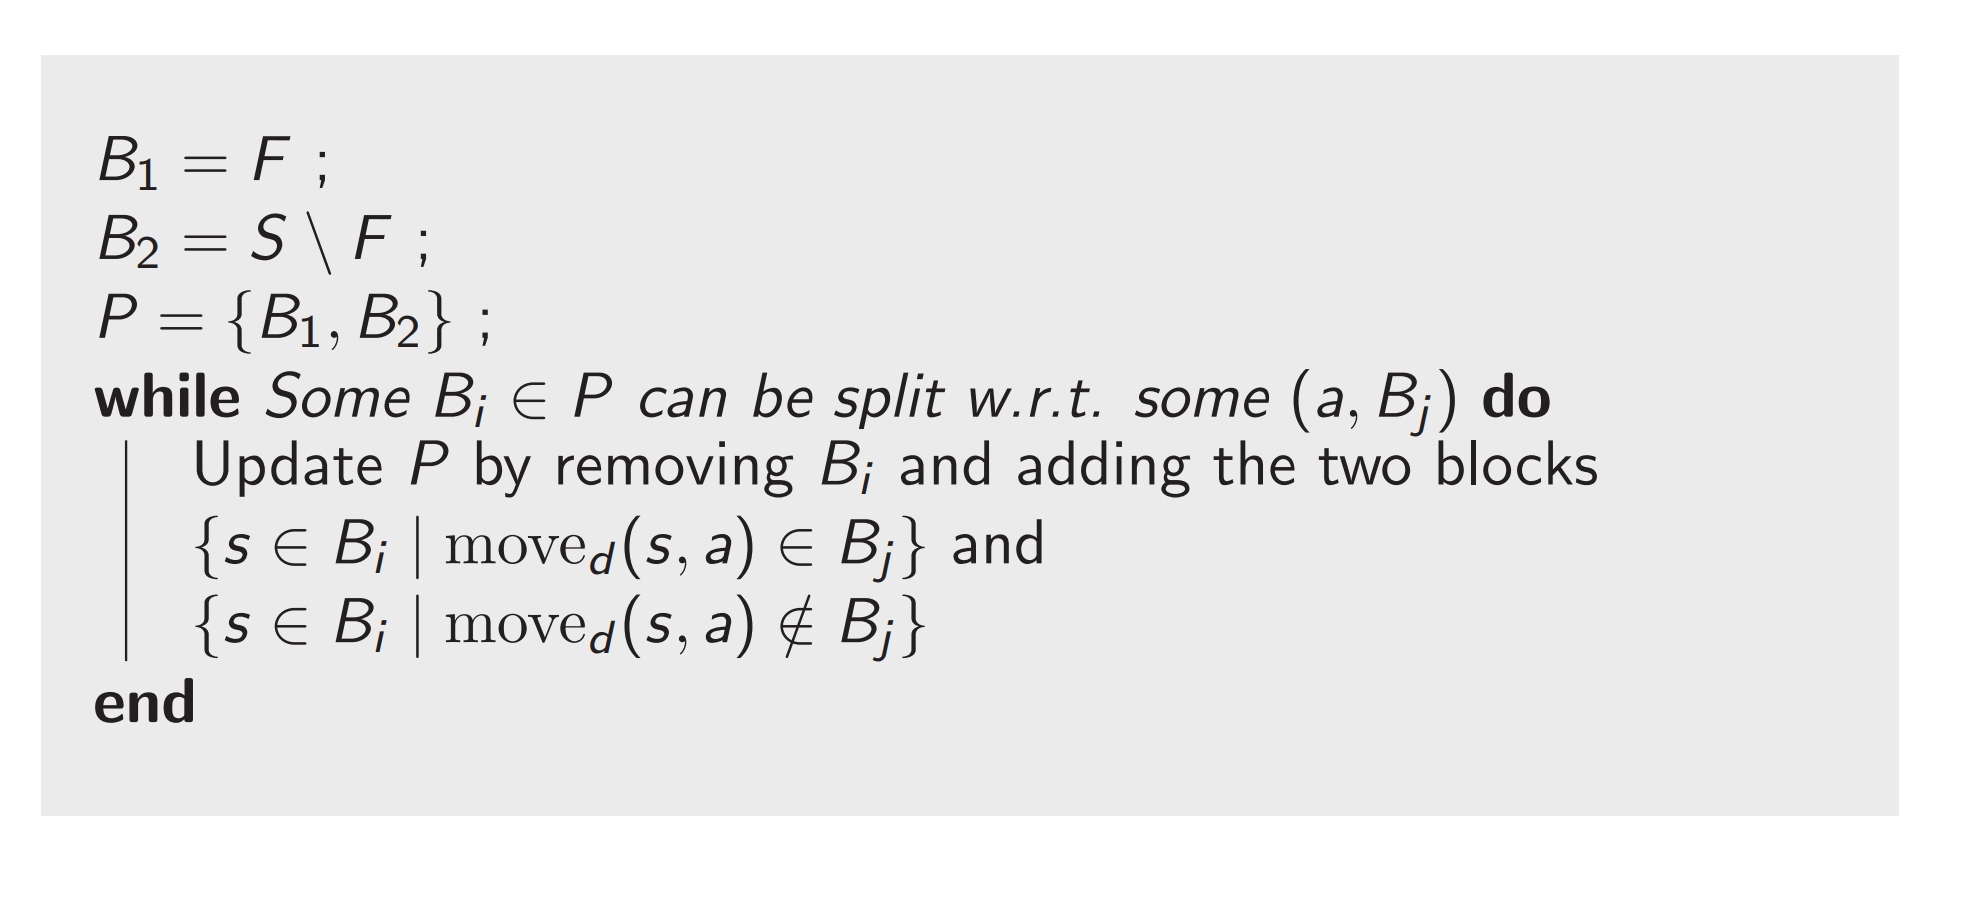
\includegraphics[width=.8\textwidth,keepaspectratio]{algoritmo partiton refinement.png}
% 	\label{partition refinement}
% 	\caption{Pseudocodice}
% \end{figure}
\subimport{assets/pseudocode/}{partition-refinement.tex}

La divisione consiste di \(B_{i}\) considerando \(a,B_{j}\) consiste nel sostituire \(B_{i}\) con due blocchi, \( B_{i1} = {s \in B_{j} | move_{d}(s,a)\in B}\) e \( B_{i2} = {s \in B_{j} | move_{d}(s,a)\notin B}\)

\subsection{Esercizi sulla minimizzazione DFA}
\subsubsection{Esercizio 1}
Passiamo ad applicare la procedura di minimizzazione ad uno degli esempi già visti in passato.

\begin{figure}[H]
	\centering
    \subimport{assets/figures/}{es1_DFA_minimization.tex}
	\caption{Esercizio 1}
	\label{mindfa-es-1}
\end{figure}

Iniziamo con due blocchi iniziali: \(B_{1}=\{E\}\), dato dallo stato finale, e \(B_{2}=\{A,B,C,D\}\). Notiamo che \((b,B_{1})\) spezza \(B_{2}\), per cui abbiamo due blocchi \(B_{21}=\{D\}\) e \(B_{22}=\{A,B,C\}\). Notiamo ancora che è possibile spezzare \(B_{22}\) in \(B_{221}=\{B\}\) e \(B_{222}=\{A,C\}\). Otteniamo quindi il DFA minimo illustrato in figura \ref{mindfa-es1-sol}. 

\begin{figure}[H]
	\centering
    \subimport{assets/figures/}{sol_es1_DFA_minimization.tex}
	\caption{Soluzione di questo primo esercizio}
  \label{mindfa-es1-sol}
\end{figure}

\subsubsection{Esercizio 2}
Proviamo con questo altro esercizio:

\begin{figure}[H]
	\centering
    \subimport{assets/figures/}{es2_DFA_minimization.tex}
	\caption{DFA dell'esercizio 2}
  \label{mindfa-es-2}
\end{figure}

In questo caso la funzione di transizione non è totale; dobbiamo quindi renderla tale aggiungendo un nodo \(sink\) a cui facciamo arrivare ogni coppia \(stato, simbolo\) mancante dall'equivalente funzione di transizione parziale.

\begin{figure}[H]
	\centering
    \subimport{assets/figures/}{es2_DFA_minimization_total_transition.tex}
	\caption{DFA dell'esercizio 2 con transizione totale}
  \label{minndfa-es-2-tot}
\end{figure}

Dopo aver realizzato questo, iniziamo con gli insiemi \(B_{1}=\{D\}\) e \(B_{2}=\{A,B,D,sink\}\). Possiamo fare uno \emph{split} di \(B_{2}\), in quanto \(\textrm{move}_{d}(A,a) \in B_{2} \) e \(\textrm{move}_{d}(B,a) \notin B_{2} \); da questo split otteniamo i nuovi blocchi \(B_{21}=\{A,sink\}\) e \(B_{22}=\{B,C\}\).

Possiamo fare un ulteriore \emph{split} di \(B_{22}\), poiché \(\textrm{move}_{d}(B,b) \in B_{22} \) e \(\textrm{move}_{d}(C,b) \notin B_{22} \); da questo otteniamo i blocchi \(B_{221}=\{B\}\) e \(B_{222}=\{C\}\).

Infine notiamo che è possibile uno \emph{split} di \(B_{21}\), dal momento che \(\textrm{move}_{d}(A,a) \in B_{221} \) e \(\textrm{move}_{d}(Sink,a) \notin B_{221} \). Otteniamo quindi i blocchi \(B_{211}=\{A\}\) e \(B_{212}=\{sink\}\).
La situazione finale diventa \(B_{1}=\{D\}\), \(B_{211}=\{A\}\), \(B_{212}=\{sink\}\), \(B_{221}=\{B\}\), \(B_{222}=\{C\}\).

Da questo eliminiamo il blocco \(B_{212}\), in quanto il blocco \emph{Sink} non trova posto nel nostro DFA minimo; notiamo però che il DFA minimo che otteniamo è identico a quello di partenza. Il DFA, infatti, era già minimo.  

\begin{figure}[H]
	\centering
    \subimport{assets/figures/}{es2_DFA_minimization.tex}
	\caption{Soluzione Esercizio 2}
  \label{mindfa-es-2-sol}
\end{figure}

\subsubsection{Esercizio 3}
Passiamo ora ad un esercizio più completo. Si richiede di trasformare l'NFA in Fig.\ref{mindfa-es-3} in un DFA e successivamente in un min DFA.
\begin{figure}[htb]
	\centering
  \subimport{assets/figures/}{nfa2.tex}
	\caption{Esercizio 3}
	\label{mindfa-es-3}
\end{figure}
Procediamo dunque, come da prassi, con lo svolgimento della procedura di subset construction per creare un DFA corrispondente. La tabella che riassume tale procedimento è riportata come Tab.\ref{mindfa-es-3-tab}.
\begin{table}[H]
	\centering
	\subimport{assets/tables/}{mindfa-es3-tbl.tex}
	\caption{Tabella per la subset construction}
	\label{mindfa-es-3-tab}
\end{table}
A questo punto dobbiamo costruirne la rappresentazione del DFA, che si può osservare in Fig.\ref{dfa-sc-es-3-mindfa}, e trovarne il minimo.
\begin{figure}
	\centering
	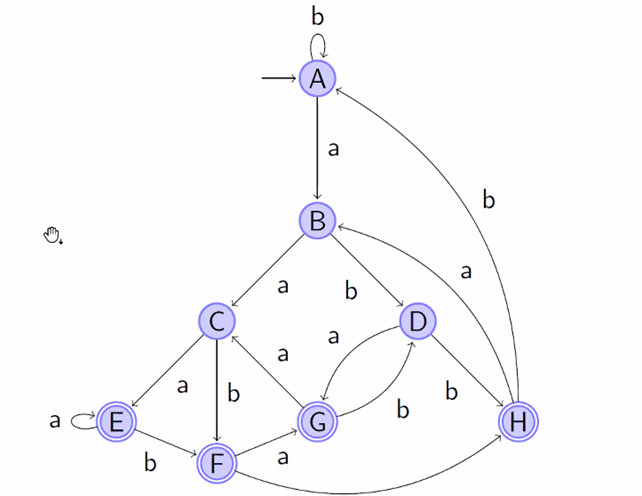
\includegraphics[width=.7\textwidth,keepaspectratio]{esercizio-min-dfa-3_dfa_da_sc.png}
	\caption{DFA ottenuto con subset construction}
	\label{dfa-sc-es-3-mindfa}
\end{figure}
Procediamo ora con l’algoritmo di partition refinement per minimizzare il precedente DFA.

Il primo passo è quello di dividere l'insieme \(S\) degli stati in due blocchi: gli stati finali (\(B2\)) e gli stati non finali (\(B1\)).
In questo caso le partizioni sono le seguenti:
\begin{equation*}
    B1 = \{A,B,C,D\} \quad \textrm{e} \quad B2 = \{E,F,G,H\}
\end{equation*}

A questo punto procediamo con le raffinazioni successive. Se all’interno dello stesso blocco troviamo due stati che, tramite una \(a\)-transizione, portano a due blocchi distinti (con \(a\) terminale qualsiasi dell’alfabeto \(\mathcal{A}\)), allora splittiamo questo blocco in due nuovi blocchi nel seguente modo:
\begin{enumerate}
    \item identifichiamo i due stati \(s_1\) e \(s_2\) che con una \(a\)-transizione portano rispettivamente uno in un blocco \(By\) e l’altro in un blocco \(Bz\);
    \item creiamo due nuovi sottoblocchi di \(Bx\): \(Bx_{1}\) conterrà tutti gli stati che da \(Bx\) arrivano a \(By\) con una \(a\)-transizione e \(Bx_{2}\) conterrà tutti gli stati in \(Bx \setminus Bx_{1}\).
\end{enumerate} 
Preme sottolineare che la scelta di quale blocco splittare influisce molto sull’efficienza dell’algoritmo, e gli algoritmi più efficienti svolgono questa scelta in maniera mirata.

Osservo che \(\textrm{move}_d (C,a)\) non ha lo stesso blocco target di \(\textrm{move}_d (A,a) \): infatti, con una \(a\)-transizione da \(A\) raggiungo \(B1\), con una \(a\)-transizione da \(C\) raggiungo \(B2\). Decido quindi di splittare \(B1\) secondo \(\textrm{move}_d (A,a) \). In questo caso il risultato della partizione è il seguente:
\begin{equation*}
    \{A, B\};\; \{C, D\};\; \{E,F,G,H\}
\end{equation*}

Questa nuova partizione è ulteriormente splittabile? Sì! Posso eseguire uno split su \(\textrm{move}_d(A, a)\), dato che attraverso una \(a\)-transizione da \(A\) mi muovo in \(\{A,B\}\), mentre da \(B\) mi muovo in \(\{C,D\}\). Splitto quindi il blocco \(\{A,B\}\) e ottengo questa nuova suddivisione:
\begin{equation*}
    \{A\};\; \{B\};\; \{C, D\};\; \{E,F,G,H\}
\end{equation*}
Ora procediamo ad oltranza con i raffinamenti successivi. Posso splittare su \(\textrm{move}_d(G,b)\) e \(\textrm{move}_d(H,b)\), ottenendo:
\begin{equation*}
    \{A\};\; \{B\};\; \{C, D\};\; \{E,F,H\};\; \{G\}
\end{equation*}
Il prossimo è lo split su \(\textrm{move}_d(C, a)\) e \(\textrm{move}_d(D, a)\), che mi porta ad ottenere:
\begin{equation*}
    \{A\};\; \{B\};\; \{C\};\; \{D\};\; \{E,F,H\};\; \{G\}
\end{equation*}
E ora splitto su \(\textrm{move}_d(E, a)\) e \(\textrm{move}_d(H, a)\):
\begin{equation*}
    \{A\};\; \{B\};\; \{C\};\; \{D\};\; \{E,F\};\; \{H\};\; \{G\}
\end{equation*}
Infine, posso splittare anche su \(\textrm{move}_d(E, a)\) ed \(\textrm{move}_d(F, a)\), arrivando quindi al raffinamento con la seguente forma:
\begin{equation*}
    \{A\};\; \{B\};\; \{C\};\; \{D\};\; \{E\};\; \{F\};\; \{H\};\; \{G\}
\end{equation*}
A questo punto ho raggiunto una partizione in cui tutti i blocchi contengono un solo stato.

In questo caso ho terminato lo svolgimento dell'algoritmo di partition refinement; questo significa che il DFA da cui sono partito (ottenuto da subset construction) era esattamente minimo.

\subsubsection[Tutta da risistemare]{Discussione: “Qual è la scelta ottimale per lo split?”}
Domanda interessante. La discussione, essendo un trivia, verrà trascritta in un secondo momento.
% L’idea alla base dell’algoritmo più efficiente è andare a splittare i blocchi che sono splittabili per archi entranti nei blocchi più piccoli.
% Un algoritmo non efficientissimo ma davvero semplice da scrivere è il seguente
% Algoritmo di Brzozowski
% % min(D) = sub_c(rev(sub_c(rev(D))))
% Precondizione: il DFA può avere un set di stati iniziali
% (non cambia molto per la sub_c: invece di avere lo stato S_0 si ha un insieme di stati T_0, di conseguenza invece che la e-chiusura di S_0 si usa la e-chiusura di T_0)
% Provando ad applicare questo algoritmo su 2/3 automi diversi si dovrebbe arrivare a capire quali sono le scelte migliori per applicare lo split.

\subsection{Dimensione di un DFA}
\begin{lemma}
    Per ogni \(n \in  \mathbb{N}^+\) esiste un NFA con \((n+1)\) stati il cui DFA minimo equivalente ha almeno \(2^n\) stati.
\end{lemma}
\begin{proof}
    Prendiamo ad esempio il linguaggio:
    \begin{equation}
        \mathcal{L} = \mathcal{L}((a\mid b)^\ast a (a\mid b)^{n-1})  
        \label{linguaggio_lemma_limiti_dfa}
    \end{equation}
    Dal momento che è un linguaggio regolare, questo può essere rappresentato utilizzando un automa a stati finiti. Esiste un NFA con esattamente \(n+1\) stati che accetta il linguaggio \(\mathcal{L}\); tale automa è rappresentiato in figura \ref{nfa_lemma_limiti_dfa}.
    \begin{figure}[H]
        \centering
        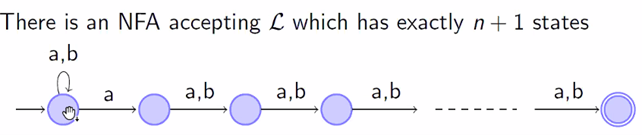
\includegraphics[width=.7\textwidth,keepaspectratio]{nfa_lemma_limiti_dfa.png}
        \caption{NFA rappresentante il linguaggio \ref{linguaggio_lemma_limiti_dfa}}
        \label{nfa_lemma_limiti_dfa}
    \end{figure}
    Supponiamo per assurdo che esista un DFA minimo, diaciamo \(\mathcal{D}\), che accetti il linguaggio \(\mathcal{L}\) ed abbia \(k<2^n\) stati.

    Sappiamo esserci esattamente \(2^n\) parole distinte su \(\{a, b\}\) la cui lunghezza è \(n\). Esistono quindi 2 percorsi in \(\mathcal{D}\) tali che:
    \begin{itemize}
        \item la loro lunghezza è \(n\);
        \item compongono rispettivamente le parole \(w_1\) e \(w_2\), con \(w_1 \neq w_2\);
        \item condividono almeno un arco.
    \end{itemize}
    Se non esistesser0,o allora i nodi sarebbero proprio \(2^n\); di conseguenza per qualche \(x_1\), \(x_2\) e \(x\) vale una delle due opzioni seguenti:
    \begin{enumerate}
        \item \(w_1 = x_1 a x \quad \textrm{e} \quad w_2 = x_2 b x\)
        \item \(w_1 = x_1 b x \quad \textrm{e} \quad w_2 = x_2 a x\)
    \end{enumerate}
    altrimenti le due parole \(w_1\) e \(w_2\) sarebbero uguali.\\
    Supponiamo in questo caso che sia valida la condizione:
    \begin{equation*}
        w_1 = x_1 a x \quad \textrm{e} \quad w_2 = x_2 b x
    \end{equation*}
    Allora possiamo definire \(w_1'\) in questo modo:
    \begin{equation*}
        w_1' = x_1 a b^{n-1} \in \mathcal{L}(\mathcal{D})
    \end{equation*}
    Di conseguenza, lo stato nuovamente aggiunto da \(w_1'\) in \(\mathcal{D}\) è uno stato finale.
    La precedente affermazione è una contraddizione: lo stato non può essere finale, perché può essere raggiunto anche tramite \(x_2 b b^{n-1}\), ma 
    \begin{equation*}
        x_2 b b^{n-1} \notin \mathcal{L}(\mathcal{D})
    \end{equation*}
    questo è l'assurdo che prova la validità del lemma.
\end{proof}
Tutto il lemma gioca sul fatto che un DFA ha bisogno esattamente di tutti i possibili cammini che siano composti da \(n-1\) alternanze di \(a\) e di \(b\) per esprimere lo stesso linguaggio espresso dall'NFA.

Questo lemma quindi ci offre una stima per il numero minimo di stati di un DFA che rappresenta un certo altro NFA.

\subsubsection{Pumping Lemma per linguaggi regolari}
\begin{lemma}
    Sia \(\mathcal{L}\) un linguaggio regolare; allora vale che:
    \begin{itemize}
        \item \(\exists p \in \mathbb{N}^+\) tale che 
        \item \(\forall z \in \mathcal{L}\) tali che \(|z|>p\)
        \item \(\exists \;u, v, w\) tale che
        \begin{itemize}
            \item \(z = uvw\)  e
            \item \(|uv| \le p\)  e
            \item \(|v| \ge 0\)  e
            \item \(\forall i \in \mathbb{N} \; . \; uv^iw \in \mathcal{L}\)
        \end{itemize}
    \end{itemize}
\end{lemma}
\noindent Ovvero, come il lettore avrà ben notato, questo è il corrispettivo del pumping lemma per i linguaggi regolari. Illustriamo ora la dimostrazione di questo lemma.
\begin{proof}
    Dato che \(\mathcal{L}\) è un linguaggio regolare, sappiamo che esiste un DFA \(\mathcal{D} = (S,\mathcal{A},\textrm{move}_d ,s_0, F)\) tale per cui \(\mathcal{L} = \mathcal{L}(\mathcal{D})\).

    Fissiamo quindi \(p=|S|-1\); ciò significa che tutti i cammini che partono da \(s_0\) ed arrivano ad uno stato finale, passando per ogni stato al massimo una volta, hanno lunghezza limitata da \(p\).

    Quindi, se per una parola \(z\) vale \(|z|>p\), allora possiamo scomporre \(z\) in \(z = a_1 \dots a_p z'\) e abbiamo la certezza che almeno uno stato, diciamo \(s^\ast\), sia attraversato più di una volta lungo il cammino \(a_1 \dots a_p\).

    Questo significa che esiste un ciclo in \(\mathcal{D}\) che parte da \(s^\ast\) e torna in \(s^\ast\), e questo ciclo si può indicare come \(a_{i+1} \dots a_j\), con \(i<j\le p\).

    Definiamo ora \(u\), \(v\) e \(w\):
    \begin{itemize}
        \item \(u = a_1 \dots a_i\)
        \item \(v = a_{i+1} \dots a_j\),  (quindi \(v\) rappresenta il ciclo)
        \item \(w = 
        \begin{cases}
            z'                   & \textrm{se} \ j = p\\ 
            a_{j+1} \dots a_pz'  & \textrm{se} \ j < p
        \end{cases}\)
    \end{itemize}

    Quindi possiamo tranquillamente affermare che \(|uv| \le p\) e che la lunghezza di \(v\) è almeno \(1\) (per definizione un ciclo ha almeno un nodo). Inoltre, essendo \(v\) il ciclo, esso è ripetibile (pumping) un numero indefinito di volte, con la garanzia che \(uv^iw\) sia accettato da \(\mathcal{D}\) per ogni valore \(i \in \mathbb{N}\). 
\end{proof}
Abbiamo quindi dimostrato questa versione del pumping lemma per i linguaggi regolari, ora la domanda che sorge spontanea è: per cosa si utilizza questo lemma? Come nel caso dei linguaggi liberi, questo lemma viene utilizzato per dimostrare, tramite contraddizione, che un certo linguaggio \emph{non} è regolare. Quindi, si assume che un dato linguaggio \(\mathcal{L}\) sia regolare, e se si riesce a dimostrare che per quel linguaggio la tesi non è soddisfatta (ovvero il negato della tesi è soddisfatto), allora si può affermare che \(\mathcal{L}\) in realtà non è un linguaggio regolare.

Ripetiamo la tesi, per amor di chiarezza, e ne scriviamo in seguito la negazione.
\begin{labeling}{Negato}
    \item[Tesi] 
    \(\exists p \in \mathbb{N}^+ . \;\forall z \in \mathcal{L}:|z|>p . \; \exists \;u, v, w . \; P\), \\ 
    dove \\
    \(P \equiv (z = uvw \textrm{ and } |uv| \le p \textrm{ and } |v| \ge 0 \textrm{ and } \forall i \in \mathbb{N} . \; uv^iw \in \mathcal{L}) \)
    \item[Negato]
    \(\forall p \in \mathbb{N}^+ . \;\exists z \in \mathcal{L}:|z|>p . \; \forall \;u, v, w . \; Q\), \\
    dove \\
    \(Q \equiv (z = uvw \textrm{ and } |uv| \le p \textrm{ and } |v| \ge 0) \implies (\exists i \in \mathbb{N} . \; uv^iw \notin \mathcal{L}) \) 
\end{labeling}

\subsubsection{Applicazioni del pumping lemma per linguaggi regolari}
Vediamo subito come possiamo applicare il lemma per dimostrare la seguente affermazione:
\begin{equation}
    \mathcal{L} = \{a^n b^n \mid n>0\} \quad \textrm{non è regolare.}
    \label{pl_regular_languages_ex_1}
\end{equation}
Prima di proseguire con la dimostrazione formale, proviamo a spiegare che intuizione potrebbe dirci che ci troviamo davanti ad un linguaggio non regolare.

Se \(\mathcal{L}\) fosse un linguaggio regolare dovrebbe essere possbile rappresentarlo con un NFA o un DFA. Proviamo quindi a immaginare il DFA che riconosce questo linguaggio, come dovrebbe essere? Per bilanciare il numero di \(b\) e di \(a\) dovrebbe in qualche modo obbligare l’inserimento di una \(b\) per ogni \(a\) inserita in precedenza, ma questo non si può fare a meno di inserire infiniti stati, il che è impossibile.

Procediamo quindi con la dimostrazione tramite pumping lemma. Supponiamo \(\mathcal{L}\) regolare e prendiamo \(p\) intero positivo arbitrario (il negato della tesi deve valere per ogni \(p\)). Ora, costruiamo la parola \(z=a^p b^p\); abbiamo che \(|z|>p\).
Osserviamo che:
\begin{equation*}
    \forall \; u,v,w \ \textrm{se} \ (z = uvw \quad \textrm{e} \quad |uv| \le p \quad \textrm{e} \quad |v| > 0)
\end{equation*}
Sappiamo inoltre che:
\begin{itemize}
    \item la componente \(v\) contiene almeno una \(a\) (da \(|v| > 0\));
    \item la componente \(v\) può contenere solamente \(a\) (altrimenti violerebbe \(|uv| \le p\)).
\end{itemize}
Se noi ora definiamo \(j > 0\) tale per cui 
\begin{equation*}
    uv^2w = a^pa^jb^p 
\end{equation*}
abbiamo che \(uv^2w \notin \mathcal{L}\), il che contraddice il pumping lemma per i linguaggi regolari.

Abbiamo quindi dimostrato per contraddizione del pumping lemma per linguaggi regolari che l'affermazione in equazione \ref{pl_regular_languages_ex_1} è verificata.

\section{Training}
\subsection{Esercizio 1}
Sia \(\mathcal{L}_1\) il linguaggio delle parole su \(\{a, b\}\) con un numero dispari di occorrenze di \(b\). \(\mathcal{L}_1\) è regolare?

Proponiamo di seguito delle espressioni regolari e dei DFA che sono stati selezionati durante la lezione con una breve spiegazione a riguardo 

\begin{itemize}
    \item l'espressione regolare \((a^*(bb)^*)^* b(a^*(bb)^*)^*\) non può denotare il linguaggio descritto poiché \(ababab \notin \mathcal{L}_1\).
    \item definiamo un automa con due stati \(A\) iniziale e \(B\) finale. \(A\) presenta una \(a\)-transizione in \(A\) ed una \(b\)-transizione in \(B\) mentre \(B\) ha una \(a\)-transizione in \(B\) e una \(b\)-transizione in \(A\). Notare che lo stato \(A\) rappresenta il caso in cui sono state lette un numero pari di \(b\) mentre \(B\) quello in cui sono state lette un numero dispari di \(b\): nel caso iniziale, infatti, si è obbligati ad aggiungere almeno una \(b\) per raggiungere lo stato finale ma, nel caso in cui si voglia aggiungere un'altra \(b\), è necessario ritornare nello stato \(A\) e rifare il procedimento descritto. Considerando che in entrambi gli stati è possibile mettere un numero arbitrario di \(a\), possiamo dichiarare questa soluzione come corretta.
    \item l'espressione regolare \((a^*(b)a^*)(a^*(b)a^*(b)a^*)^*\) sembrerebbe essere corretta in quanto sicuramente accetterò parole composte da almeno una \(b\) e un numero arbitrario di \(a\) prima e dopo; nel caso in cui volessi aumentare il numero di \(b\), sono obbligato a farlo a coppie con la possibilità di interporre un numero arbitrario di \(a\) prima, in mezzo o alla fine. 
\end{itemize}

In questo caso, visto che siamo stati in grado di trovare un DFA con un numero finito di stati, possiamo affermare che \(\mathcal{L}_1\) è un linguaggio regolare. Come possiamo però essere certi del fatto che, ad esempio, l'espressione regolare \((a^*(b)a^*)(a^*(b)a^*(b)a^*)^*\) denoti il linguaggio \(\mathcal{L}_1\) e che quindi sia anch'essa soluzione al quesito? Il modo corretto di procedere è il seguente:

\begin{enumerate}
    \item si utilizza la \emph{Thompson's Construction} per generare l'NFA corrispondente;
    \item si applica l'algoritmo di \emph{Subset Construction} per trasformare l'NFA in un DFA;
    \item si applica l'algoritmo per la \emph{DFA minimization} (aggiungendo dunque lo stato sink se necessario) per ridurre il numero di stati;
    \item si osserva se il DFA ridotto è in realtà un isomorfismo del DFA proposto come soluzione.
\end{enumerate}

\noindent Notare che in questo caso una soluzione possibile (proposta dalla professoressa) è \((b a^*b \mid a)^* ba^*\)

\subsection{Esercizio 2}
Sia \(\mathcal{L}_2\) il linguaggio delle parole su \(\{a, b\}\) con un numero pari di occorrenze di \(a\). \(\mathcal{L}_2\) è regolare?

Per rispondere a tale quesito si potrebbe pensare di costruire un DFA con lo stesso ragionamento di prima: uno stato il caso in cui le occorrenze di \(a\) sono pari mentre l'altro in cui sono dispari.

Poiché \(0\) è considerato pari, in questo caso lo stato iniziale coincide con quello finale. Le transizioni devono essere opportunamente costruite, per cui se voglio aggiungere una \(a\) alla mia parola sono costretto a seguire una \(a\)-transizione in uno stato non finale per poi tornare in quello finale con un'ulteriore \(a\)-transizione, in modo da assicurare che le condizioni siano rispettate. Ovviamente, deve esservi sempre la possibilità di inserire un numero arbitrario di \(b\) tra le varie occorrenze di \(a\), per cui in entrambi gli stati si ha una \(b\)-transizione sullo stesso stato. Analogamente all'esercizio precedente si ha che \(\mathcal{L}_2\) è un linguaggio regolare. In questo caso l'espressione regolare proposta è stata \((b^*ab^*ab^*)^*\) .
% (P.S. ho provato a fare l'isomorfismo di questo grafo e non viene mai nella vita identico a quello precedente, potrei avere tranquillamente sbagliato ma l'abbiamo fatto in 3 e non risulta quindi o c'è qualcosa che mi sfugge o IDK)

\subsection{Esercizio 3}  
Sia \(\mathcal{L}_3\) il linguaggio delle parole su \(\{a, b\}\) con un numero dispari di occorrenze di \(b\) \textbf{oppure} un numero pari di occorrenze di \(a\). \(\mathcal{L}_3\) è regolare?

Una soluzione tanto banale quanto efficace consiste nel utilizzare la Thompson's Construction per poter concatenare gli automi descritti negli esercizi precedenti con l'operazione di \emph{Alternation}. A livello formale questo si traduce come:
\begin{equation*}
    \mathcal{L}(r_1 \mid r_2) = \mathcal{L}(r_1) \cup \mathcal{L}(r_2)
\end{equation*}
Essendo che \(\mathcal{L}_1\) e \(\mathcal{L}_2\) sono linguaggi regolari, l'unione dei due così descritta non può che essere anch'essa un linguaggio regolare.

Nel caso in cui fosse stato richiesto di verificare un linguaggio dove valessero \textbf{entrambe} le condizioni precedenti avremmo dovuto procedere in modo diverso. Sono dati i seguenti casi:
\begin{itemize}
    \item abbiamo un numero di \(a\) pari e di \(b\) pari;
    \item abbiamo un numero di \(a\) pari e di \(b\) dispari;
    \item abbiamo un numero di \(a\) dispari e di \(b\) pari;
    \item abbiamo un numero di \(a\) dispari e di \(b\) dispari.
\end{itemize}
Ovviamente il nostro stato iniziale non può essere altro che quello dove si hanno \(0\) occorrenze di \(a\) e di \(b\) (il primo descritto), mentre lo stato finale dovrà per forza essere il secondo dell'elenco. Dunque quello che abbiamo appena immaginato di costruire è un'automa che possiede \(4\) possibili stati di cui soltanto uno deve essere considerato quello finale. 

Sicuramente l'idea precedente è corretta, ma c'era un altro modo per arrivare direttamente alla soluzione senza dover fare un ragionamento di quel tipo, ma pensando invece all'intersezione: immaginiamo di avere una parola \(w\) a disposizione e di poterci contemporaneamente muovere su entrambi i cammini degli automi descritti come soluzioni di \(\mathcal{L}_1\) e di \(\mathcal{L}_2\). Continuiamo a spostarci eseguendo le transizioni coerentemente alla parola \(w\) scelta, fino a che non arriviamo al carattere terminatore. A questo punto sono dati due casi:
\begin{enumerate}
    \item se mi trovo in entrambi gli automi su uno stato finale allora \(w \in \mathcal{L}\)
    \item se uno dei due stati su cui mi trovo non è uno stato finale allora \(w \notin \mathcal{L}\)
\end{enumerate}
Per poter semplificare la procedura possiamo immaginare di fare il prodotto cartesiano degli stati dei due automi.

\section{Proprietà di chiusura nei linguaggi regolari}

I linguaggi regolari sono chiusi rispetto alle seguenti operazioni:
\begin{itemize}
	\item unione;
	\item concatenazione;
	\item complementazione;
	\item intersezione.
\end{itemize}
Andiamo a vedere più da vicino le motivazioni per ciascuna di queste.

\paragraph{Unione}
Se prendiamo due linguaggi regolari e ne operiamo l'unione, il risultato di questa è ancora un linguaggio regolare. Come nel caso precedente, essendo che i linguaggi sono regolari, allora è possibile costruire un DFA sia per il primo che per il secondo; se a questo punto si prendono i due automi così costruiti e li si lega tramite una \(\epsilon\)-transizione, per l'operazione di \emph{Alternation} si ottiene nuovamente 
un linguaggio regolare.

\paragraph{Concatenazione}
È possibile eseguire l'operazione di \emph{Concatenation} della Thompson's Construction e ottenere ancora una volta un'automa che denota un linguaggio regolare.

\paragraph{Complementazione}
Se \(\mathcal{L}\) è un linguaggio regolare su un certo alfabeto \(\mathcal{A}\), la complementazione è data dal linguaggio delle parole su \(\mathcal{A} \setminus \mathcal{L}\). Se un linguaggio è regolare allora anche il suo complemento è regolare. 

\paragraph{Intersezione}
È derivabile dall'unione utilizzando le regole di \emph{De Morgan}: 
\begin{equation*}
    \mathcal{L}_1 \cap \mathcal{L}_2 = \lnot (\lnot (L1 \cap L2)) = \lnot (\lnot \mathcal{L}_1 \cup \lnot \mathcal{L}_2)
\end{equation*}

In precedenza abbiamo visto l'automa che riconosce \(\mathcal{L}_2\), ovvero che accetta tutte quelle parole dove \(a\) occorre un numero pari di volte. Il complementare di tale automa corrisponde a quello per cui si hanno parole con un numero dispari di occorrenze. Utilizzando l'automa che denota \(\mathcal{L}_2\), vi è la possibilità di applicare una particolare operazione per trasformarlo nel suo complementare? Sì, è possibile: basta semplicemente rendere finali tutti quegli stati che prima non lo erano e, simmetricamente, non finali tutti quelli che prima lo erano.

Relativamente questo procedimento è però necessario fare una precisazione: tale metodo funziona solamente se il DFA presenta una funzione di transizione \textbf{totale}: intuitivamente, è necessario riconoscere tutte quelle parole che non appartengono al linguaggio regolare in quanto queste apparterranno al linguaggio del DFA complementare; se per assurdo si avesse la mancanza di una \(a\)-transizione (non fondamentale nel primo DFA) non si avrebbe la possibilità di costruire il set completo delle parole.

\end{document}
